% Paper 2: Tiled DP-Splat for UAV Mapping (IEEE TGRS submission draft)
% Compile: cd paper && tectonic main.tex
\documentclass[journal]{IEEEtran}

\usepackage[T1]{fontenc}
\usepackage{microtype}
\usepackage{amsmath,amssymb}
\usepackage{graphicx}
\usepackage{tikz}
\usetikzlibrary{calc,arrows.meta}
\usepackage{cite}
\usepackage[hidelinks]{hyperref}

\interdisplaylinepenalty=2500

% Reporting thresholds only (no layout effect): underfull-box reports are
% cosmetic in two-column IEEEtran with \looseness=-1 paragraphs; suppress
% them while leaving overfull detection (\hfuzz, \vfuzz) untouched.
\hbadness=10000
\vbadness=10000

% Vertical-space discipline (page-budget pass): modestly tighter float and
% display spacing; no content or font-size changes.
\setlength{\textfloatsep}{0.8\baselineskip plus 0.2\baselineskip minus 0.3\baselineskip}
\setlength{\dbltextfloatsep}{0.8\baselineskip plus 0.2\baselineskip minus 0.3\baselineskip}
\setlength{\floatsep}{0.65\baselineskip plus 0.2\baselineskip minus 0.2\baselineskip}
\makeatletter
% IEEEtran's \normalsize re-sets display skips at every size switch, so the
% override must ride along with it.
\g@addto@macro\normalsize{%
  \abovedisplayskip 4pt plus 2pt minus 2pt%
  \belowdisplayskip 4pt plus 2pt minus 2pt%
  \abovedisplayshortskip 2pt plus 1pt%
  \belowdisplayshortskip 2pt plus 1pt minus 1pt%
}
\makeatother

\begin{document}
\bstctlcite{BSTcontrol}

\title{Tiled Dirichlet-Process Gaussian Splatting for UAV Mapping with
Calibrated Uncertainty}

\author{Aqi~Dong%
\thanks{Manuscript received July~2026.}%
\thanks{A.~Dong is with the Department of Management, Marketing and
Operations, David B. O'Maley College of Business, Embry-Riddle Aeronautical
University, Daytona Beach, FL 32114 USA (e-mail: donga2@erau.edu;
ORCID: 0009-0004-1676-3528).}}

\markboth{IEEE Transactions on Geoscience and Remote Sensing}%
{Dong: Tiled Dirichlet-Process Gaussian Splatting for UAV Mapping with Calibrated Uncertainty}

\maketitle

\begin{abstract}
\looseness=-1 Operational aerial-mapping decisions need trustworthy,
spatially resolved uncertainty at survey scale. We present a fully Bayesian treatment of tiled
large-scene splatting: independent Dirichlet-process Gaussian-mixture fits
per tile are matched and merged exactly in closed form, then
stitched by a partition-of-unity
gate into one \emph{normalized}, provenance-preserving scene-level
predictive density, evaluated as a density, never as a
renderer. On three Hessigheim 3D (H3D)
LiDAR epochs (59--129 million points), that density matches the hard
seam-deletion rules of current practice to within
$0.02$--$0.03$~nats per held-out point
while deleting nothing. The normalized posterior is then spent:
coverage at 68/90/95\% is near-nominal on
H3D (68\% seam-band coverage $0.64$--$0.67$); at a second site,
all-points coverage replicates
but seam coverage falls to $0.57$. Predictive
log-density ranks held-out error better than random
(area under the sparsification error curve, AUSE, 0.16--0.20) but a model-free local-density ranker does better
still, so we claim the uncertainty as a
compact, calibrated, density-faithful surrogate, not as ranking
power beyond sampling density; predictive confidence nonetheless
stratifies mesh-referenced error monotonically. A
null-calibrated model-derived level of detection holds its
nominal level on stable ground (4.2\% vs.\ nominal 5\%;
AUC 0.72) where a same-grid classical DEM-of-difference
baseline flags 17--90\% of the same cells, though the
classical test remains the sharper pure ranker (AUC 0.82--0.97); the
${\approx}1$~m detection floor is a stated representation limit. In
re-flight planning, posterior uncertainty matches a per-tile error
oracle and beats a mass-only planner on comparable-mass tiles
($+1.10$ vs.\ $+0.86$~nats); where mass separates tiles, mass alone
plans as well. The pipeline is CPU-only: a laptop fits
152 million points in 2{,}346~s.
\end{abstract}

\begin{IEEEkeywords}
Change detection, Dirichlet process, Gaussian splatting, LiDAR, UAV
mapping, uncertainty quantification, variational inference.
\end{IEEEkeywords}

\IEEEpeerreviewmaketitle

\section{Introduction}
\label{sec:intro}

\looseness=-1 Aerial mapping products increasingly feed operational
decisions (infrastructure inspection, multi-epoch change monitoring,
follow-up flight planning) that consume a reconstruction and then act
on it. What they need is not photorealism but \emph{trustworthy, spatially
resolved uncertainty} at survey scale ($10^{8}$ points per campaign)
on hardware a field team actually has. \looseness=-1 Current practice supplies neither.
Survey-scale scenes force partitioned processing, and the dominant large-scale
splatting and neural-field pipelines resolve the resulting tile seams by
geometric heuristics: hard cropping of out-of-tile primitives~\cite{lin2024vastgaussian,liu2024citygaussian,kerbl2024hierarchical},
unweighted consensus averaging~\cite{chen2024dogs}, or hand-tuned
image-space distance blending~\cite{tancik2022blocknerf}. As a result, no
normalized global
predictive density is defined, no contribution is weighted by posterior
uncertainty, and duplicated boundary structure is deleted, never fused
(Sec.~\ref{sec:related}). Uncertainty, where it appears at all, is a post hoc
overlay on a photometric optimizer~\cite{jia2026bayesian}, not a
property of a generative model that can be calibrated and then spent.

\looseness=-1 This paper closes that gap for point-cloud splatting. Building on the
DP-Splat model~\cite{dong2026dpsplat}, a conjugate Dirichlet-process
(DP) mixture over colored points fitted by closed-form coordinate
ascent, we
develop a fully Bayesian treatment of \emph{tiled} large-scene fitting.
In one sentence: partition-of-unity stitching with exact conjugate
merging turns independent tile posteriors into one coherent,
\emph{normalized}, calibrated predictive density (at parity with hard
crop/Voronoi deletion on predictive quality, but, unlike them, a
well-defined probability model of the whole scene), and that density is
what tells the operator where the reconstruction cannot be trusted, and
where to fly next. Our contributions:
\begin{enumerate}
\item \textbf{Tiled conjugate inference with exact merging.} A partitioned
  DP-Splat pipeline: halo down-weighting, per-tile concentration bookkeeping
  ($\sum_t \alpha_t = \alpha$), Hungarian matching of straddling
  components under a normal--inverse--Wishart (NIW)
  marginal-likelihood score with exact prior-subtracted merging,
  and partition-of-unity stitching
  (Sec.~\ref{sec:method}). The matcher fires at production capacity,
  fusing, with exact provenance, the straddling structure that hard
  seam rules simply delete (Sec.~\ref{sec:results}).
\item \textbf{A held-out, seam-aware evaluation, reported at parity.}
  To our knowledge, the first exact-conjugate-generative treatment of
  tiled large-scene splatting evaluated as a scene-level predictive
  density. On three Hessigheim 3D (H3D) epochs the stitched predictive
  matches the crop and Voronoi baselines to within $0.02$--$0.03$~nats
  per held-out point (hard deletion is empirically near-costless
  here) while uniquely yielding a global density normalized up to a
  measured $0.020$ tail deficit (mass $0.980$ by numerical
  integration, Sec.~\ref{sec:setup:metrics}). Credible intervals are calibrated at
  production capacity including within the seam bands on the H3D
  epochs; at the second site, all-points calibration replicates but
  seam-band calibration does not. The merge contributes exact
  model-order de-duplication and, by ablation, $+0.14$--$0.35$~nats of
  seam log-predictive across the three epochs (Sec.~\ref{sec:results}).
\item \textbf{Uncertainty that is calibrated and then spent}, on three
  remote-sensing tasks, each with its controls measured
  (Sec.~\ref{sec:results}). In error sparsification, the predictive
  negative log-density (NLPD) ranks held-out error better than random
  on real LiDAR but is outranked by a model-free local-density
  control, so we read the signal as a compact, calibrated,
  density-faithful surrogate, not as ranking power beyond sampling
  density. Null-calibrated per-cell change detection, with a capacity
  dose--response, holds the null that a same-grid classical
  DEM-of-difference (DoD) baseline badly violates. In re-flight
  planning, posterior uncertainty matches a per-tile error oracle and
  out-plans a mass-only control where per-tile recoverable mass is
  comparable; where it is not, mass dominates and the attribution is
  stated.
\item \textbf{Laptop-scale practicality with automatic capacity adaptation.}
  The pipeline runs on a laptop CPU at $10^{8}$-point scale (SMBU, 20
  tiles: 152M points in 2{,}346~s at the production configuration;
  169M in 863~s, 37.6~GB peak, at the lighter reference arm, whose
  smaller per-tile budget explains the shorter time on more points),
  and the inferred per-tile
  component count $\hat{K}$ adapts capacity to data
  volume, deconfounded explicitly: $\hat{K}$ tracks point count, not
  scene content (Secs.~\ref{sec:results}
  and~\ref{sec:discussion}).
\end{enumerate}

\looseness=-1 Throughout, claims are scaled to the evidence: the model is evaluated
as a predictive density over colored points, never as a renderer, and
where a signal carries a confound or a task hits an intrinsic floor,
the paper quantifies the limitation rather than eliding it
(Sec.~\ref{sec:discussion}).

% =========================================================================
% Section II: Related Work
% Governing docs: paper2-uav/LIT_REVIEW.md (verified references only),
% paper/OUTLINE.md §II. Reviewer-proof prior-art sentences used verbatim
% where provided. No claims outside the claims-evidence table.
% =========================================================================

\section{Related Work}
\label{sec:related}

\subsection{Tiled Large-Scale Splatting and NeRF}
\label{sec:related-tiled}

\looseness=-1 Spatial partitioning is the accepted route to city-scale
radiance-field reconstruction, and existing pipelines resolve the
resulting seams geometrically: by hard spatial cropping of
out-of-tile primitives (VastGaussian~\cite{lin2024vastgaussian},
Sec.~4.3; CityGaussian~\cite{liu2024citygaussian}, Sec.~3.2 and its
released merge script; Kerbl \emph{et~al.}'s
hierarchy~\cite{kerbl2024hierarchical}, whose Sec.~6.3 deletes a
primitive trained by one chunk when it lies nearer another, a Voronoi
cull), by ADMM consensus whose parameter average
(Eq.~8b of DOGS~\cite{chen2024dogs}) weights position, quaternion, scale,
and opacity with uniform $1/K$ over a preassigned shared set, or by
hand-tuned inverse-distance image blending
(Block-NeRF~\cite{tancik2022blocknerf}, Sec.~4.3);
Mega-NeRF~\cite{turki2022meganerf}, drawn on here for its partitioning
scheme (and, in Sec.~\ref{sec:setup}, as the source of the Mill~19
collection), answers each query by a single nearest-centroid submodule.
In every case the merge rule is geometric and heuristic: none defines a
normalized global predictive density, none weights contributions by
posterior uncertainty, and duplicated boundary primitives are deleted,
never fused. That is workable for rasterization, which carries no
normalization constraint, but untenable for a generative model whose
output must integrate to one. Two designs are direct foils
for Sec.~\ref{sec:method}: Block-NeRF's separate appearance-matching
pass shows that models fit in isolation disagree at boundaries and
must be reconciled, and DOGS's uniform $1/K$ average ignores how much
evidence each replica holds; our merge answers both at once, exactly,
by adding prior-subtracted natural parameters on the pooled evidence.

\subsection{Bayesian Splatting}
\label{sec:related-bayes}

\looseness=-1 Jia \emph{et~al.}~\cite{jia2026bayesian} attach NIW
summaries to the standard photometric 3D Gaussian splatting (3DGS)
optimizer~\cite{kerbl2023gaussian}: pseudo-counts from an opacity--volume heuristic, the
optimizer's running center as ``observation,'' the NIW scatter
statistic held at zero;
no assignments, no E-step, no joint evidence lower bound (ELBO), and
the stick-breaking weights (Sec.~\ref{sec:model-recap}) acting purely
as a pruning schedule: summaries the authors themselves call
``optimization-driven approximations'' (their Sec.~4). That concession
motivates the opposite design, an exact conjugate generative
treatment in which responsibilities, sufficient statistics, and a
monotone ELBO are the inference itself, with Jia \emph{et~al.}\ as
precedent for image-space calibration; ours is in point/density
space. VBGS~\cite{vandemaele2024vbgs} is the closest inferential
relative: a conjugate mixture on colored points fitted by
coordinate-ascent variational inference (CAVI), but with a fixed finite
component budget and no predictive use of its posterior (rendered,
not queried as a density); its additive updates stream frames into one
fixed-capacity global model, whereas we decompose space, so capacity
adapts per tile and fits parallelize.
VBGS-SLAM~\cite{zhu2026vbgsslam} propagates camera-pose uncertainty for
indoor tracking, a different quantity from the map posterior used
here. None of these systems addresses tiling, overlap mass, or
model-order semantics. The DP-Splat
model, its stick-breaking prior, and its CAVI and stochastic
variational inference (SVI) are from
our prior work~\cite{dong2026dpsplat}; this paper contributes the tiled
inference, the exact merge, the stitched predictive, and the aerial
evaluation.

\subsection{3D Gaussian Splatting for Aerial Mapping}
\label{sec:related-aerial}

\looseness=-1 Partitioned aerial 3DGS pipelines (Yan
\emph{et~al.}~\cite{yan2025aerial}; Ortho-3DGS~\cite{ortho3dgs2025};
ULSR-GS~\cite{ulsrgs2024};
ARSGaussian~\cite{arsgaussian2026};
Horizon-GS~\cite{horizongs2025}) establish tiling as the accepted route
to large scenes but handle boundaries with engineering heuristics
(auxiliary supervision, view assignment) and leave component counts
uninterpreted; benchmark studies (Atik~\cite{atik2025benchmark};
Fadilah \emph{et~al.}~\cite{fadilah2026benchmark}, who find geometric
accuracy uncorrelated with rendering quality, and whose ``3DGS-MCMC''
baseline is a densification sampler, not posterior inference) quantify
error only post hoc against a reference cloud. None performs Bayesian
inference, produces a predictive density, or attaches calibrated
uncertainty to the map itself. TreeDGS~\cite{treedgs2026} reweights
primitives by an opacity-derived reliability score, a concrete
downstream consumer of the per-component uncertainty our posterior
provides in closed form; GU-GS~\cite{ding2026gugs} realizes
``uncertainty'' as a learned mask on the training loss, with no
probabilistic semantics; and PRIMU~\cite{gottwald2025primu} predicts
per-Gaussian uncertainty with post hoc features and a per-scene
learned regressor, setting the evaluation vocabulary (area under the
sparsification error curve, AUSE; error--uncertainty
correlation) we adopt. Neither of the latter two
reports calibration, the property we evaluate directly via interval
coverage.

\subsection{Uncertainty Evaluation, Distributed Nonparametric
Inference, and Active View Selection}
\label{sec:related-eval}

\looseness=-1 Our evaluation protocol assembles established instruments:
sparsification analysis and AUSE from Ilg
\emph{et~al.}~\cite{ilg2018uncertainty}, the area-under-random-gain
metric (AURG)
of Poggi \emph{et~al.}~\cite{poggi2020uncertainty}, and, for change
detection, the M3C2 distance measure~\cite{lague2013m3c2} with the
error-propagated level of detection of
M3C2-EP~\cite{winiwarter2021m3c2ep}, which targets the pitfall
(conflating surface roughness with positional uncertainty) that our
posterior-mean covariance construction likewise avoids by design
(Sec.~\ref{sec:setup:metrics}); Huang and Qin~\cite{huang2025uncertainty}
provide the plane-fit reference-based error convention our
sparsification analysis adopts on H3D
(Sec.~\ref{sec:setup:metrics}). The
merge machinery of Sec.~\ref{sec:method} is likewise adapted, not
invented: the closed-form merge-ratio score appears in memoized
variational inference~\cite{hughes2013memoized},
partition-probability-thresholded component matching in streaming
distributed Bayesian-nonparametric
inference~\cite{campbell2015streaming}, Hungarian parameter matching in
model aggregation~\cite{yurochkin2019spahm}, precision-weighted
combination in consensus Monte Carlo~\cite{scott2016consensus}, and the
concentration bookkeeping $\sum_t \alpha_t = \alpha$ that motivates
interpreting the merged union against a single global DP in Williamson
\emph{et al.}~\cite{williamson2013parallel} (Thm.~1); kernel
stick-breaking~\cite{dunson2008kernel} anchors the tiling: in the
compact-kernel limit, spatially localized mixtures reduce to
independent per-region DPs, the regime our tiles approximate.
Finally, uncertainty-driven view selection for splatting
(GAVIS~\cite{xue2026gavis}, FisherRF~\cite{jiang2024fisherrf},
ActiveSplat~\cite{li2025activesplat}, GauSS-MI~\cite{xie2025gaussmi}) is
sequential, GPU-rasterized, photometric, and room-scale; our re-flight
problem is batch, tile-level acquisition
ranking from rasterization-free closed-form posterior scores, evaluated
by held-out predictive density on a held-back image block's
triangulated points. GAVIS argues that parameter-space
uncertainty underestimates unseen regions; a nonparametric predictive,
whose prior reverts to a fat-tailed, low-capacity regime where data are
absent, is a natural response, and we test it directly.

\section{Method}
\label{sec:method}

\begin{figure}[t]
  \centering
  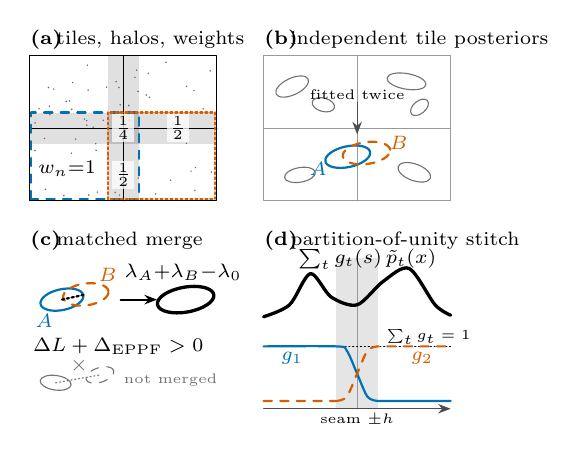
\begin{tikzpicture}[font=\scriptsize, line cap=round, line join=round,
      >={Stealth[length=1.6mm]}, scale=0.66, every node/.style={inner sep=1pt}]
    \definecolor{cbBlue}{RGB}{0,114,178}
    \definecolor{cbVerm}{RGB}{213,94,0}
    % ==== panel (a): tiling with halos ====
    \begin{scope}[shift={(0,0)}]
      \node[anchor=base west,font=\scriptsize\bfseries] at (-0.05,3.0) {(a)};
      \node[anchor=base west] at (0.45,3.0) {tiles, halos, weights};
      % halo overlap bands
      \fill[black!12] (1.5,0) rectangle (2.1,2.8);
      \fill[black!12] (0,1.1) rectangle (3.6,1.7);
      \fill[black!25] (1.5,1.1) rectangle (2.1,1.7);
      % point cloud
      \pgfmathsetseed{4242}
      \foreach \i in {1,...,60}{
        \pgfmathsetmacro{\px}{0.10+3.40*rnd}
        \pgfmathsetmacro{\py}{0.10+2.60*rnd}
        \fill[black!60] (\px,\py) circle (0.45pt);
      }
      % scene box and core grid
      \draw[black,thin] (0,0) rectangle (3.6,2.8);
      \draw[black,thin] (1.8,0) -- (1.8,2.8);
      \draw[black,thin] (0,1.4) -- (3.6,1.4);
      % two dilated (halo) tiles
      \draw[cbBlue,thick,dashed] (0.03,0.03) rectangle (2.1,1.7);
      \draw[cbVerm,thick,densely dotted] (1.5,0.03) rectangle (3.57,1.7);
      % ownership weights
      \node[fill=white,fill opacity=0.75,text opacity=1] at (0.72,0.62) {$w_n{=}1$};
      \node[fill=white,fill opacity=0.75,text opacity=1] at (1.8,0.5) {$\tfrac12$};
      \node[fill=white,fill opacity=0.75,text opacity=1] at (1.8,1.4) {$\tfrac14$};
      \node[fill=white,fill opacity=0.75,text opacity=1] at (2.85,1.4) {$\tfrac12$};
    \end{scope}
    % ==== panel (b): independent tile fits ====
    \begin{scope}[shift={(4.5,0)}]
      \node[anchor=base west,font=\scriptsize\bfseries] at (-0.05,3.0) {(b)};
      \node[anchor=base west] at (0.45,3.0) {independent tile posteriors};
      \draw[black!40,thin] (0,0) rectangle (3.6,2.8);
      \draw[black!40,thin] (1.8,0) -- (1.8,2.8);
      \draw[black!40,thin] (0,1.4) -- (3.6,1.4);
      % interior components (gray)
      \draw[black!55] (0.55,2.2) ellipse [x radius=0.34, y radius=0.16, rotate=25];
      \draw[black!55] (1.15,1.85) ellipse [x radius=0.22, y radius=0.13, rotate=-15];
      \draw[black!55] (2.75,2.3) ellipse [x radius=0.38, y radius=0.15, rotate=-10];
      \draw[black!55] (3.0,1.8) ellipse [x radius=0.2, y radius=0.12, rotate=40];
      \draw[black!55] (0.7,0.5) ellipse [x radius=0.3, y radius=0.14, rotate=10];
      \draw[black!55] (2.9,0.55) ellipse [x radius=0.33, y radius=0.16, rotate=-20];
      % one structure straddling the vertical seam, fitted twice
      \draw[cbBlue,thick] (1.62,0.85) ellipse [x radius=0.44, y radius=0.2, rotate=12];
      \draw[cbVerm,thick,dashed] (1.98,0.92) ellipse [x radius=0.46, y radius=0.21, rotate=8];
      \node[cbBlue] at (1.05,0.62) {$A$};
      \node[cbVerm] at (2.6,1.12) {$B$};
      \node[align=center] at (1.8,2.05) {\tiny fitted twice};
      \draw[->,black!70,thin] (1.8,1.9) -- (1.8,1.28);
    \end{scope}
    % ==== panel (c): Hungarian match + exact merge ====
    \begin{scope}[shift={(0,-3.85)}]
      \node[anchor=base west,font=\scriptsize\bfseries] at (-0.05,3.0) {(c)};
      \node[anchor=base west] at (0.45,3.0) {matched merge};
      % candidate pair
      \draw[cbBlue,thick] (0.62,1.95) ellipse [x radius=0.42, y radius=0.2, rotate=12];
      \draw[cbVerm,thick,dashed] (1.08,2.05) ellipse [x radius=0.44, y radius=0.21, rotate=8];
      \node[cbBlue] at (0.28,1.55) {$A$};
      \node[cbVerm] at (1.5,2.42) {$B$};
      \draw[black,densely dotted,thick] (0.62,1.95) -- (1.08,2.05);
      \node[anchor=west,align=left] at (0.0,1.05)
        {$\Delta L + \Delta_{\mathrm{EPPF}} > 0$};
      % rejected pair
      \draw[black!55] (0.5,0.35) ellipse [x radius=0.3, y radius=0.14, rotate=-8];
      \draw[black!55,dashed] (1.35,0.5) ellipse [x radius=0.28, y radius=0.14, rotate=18];
      \draw[black!55,densely dotted] (0.5,0.35) -- (1.35,0.5);
      \node[black!55] at (0.95,0.68) {$\times$};
      \node[black!55,anchor=west] at (1.75,0.4) {\tiny not merged};
      % arrow to merged component
      \draw[->,thick] (1.75,1.95) -- (2.45,1.95);
      \draw[black,very thick] (3.0,1.95) ellipse [x radius=0.55, y radius=0.24, rotate=10];
      \node[anchor=south,align=center] at (2.95,2.26)
        {$\lambda_A{+}\lambda_B{-}\lambda_0$};
    \end{scope}
    % ==== panel (d): partition-of-unity stitching ====
    \begin{scope}[shift={(4.5,-3.85)}]
      \node[anchor=base west,font=\scriptsize\bfseries] at (-0.05,3.0) {(d)};
      \node[anchor=base west] at (0.45,3.0) {partition-of-unity stitch};
      % halo band
      \fill[black!10] (1.4,-0.15) rectangle (2.2,2.75);
      \draw[black!40,thin] (1.8,-0.15) -- (1.8,2.75);
      % stitched density (upper): convex blend across the seam
      \draw[black,very thick]
        plot[smooth] coordinates {(0,1.62) (0.5,1.85) (0.9,2.45) (1.3,2.0)
          (1.8,1.85) (2.3,2.3) (2.8,2.55) (3.3,1.85) (3.6,1.65)};
      \node[anchor=west] at (0.6,2.72) {$\sum_t g_t(s)\,\tilde p_t(x)$};
      % gates (lower)
      \draw[->,black!70,thin] (0,-0.15) -- (3.6,-0.15);
      \draw[black,densely dotted] (0,1.05) -- (3.6,1.05);
      \node[anchor=south west] at (2.32,1.02) {\tiny $\sum_t g_t = 1$};
      \draw[cbBlue,thick]
        plot[smooth] coordinates {(0,1.05) (1.4,1.05) (1.6,0.97) (1.8,0.525)
          (2.0,0.08) (2.2,0.0)} -- (3.6,0);
      \draw[cbVerm,thick,dashed] (0,0) -- (1.4,0)
        plot[smooth] coordinates {(1.4,0.0) (1.6,0.08) (1.8,0.525)
          (2.0,0.97) (2.2,1.05)} -- (3.6,1.05);
      \node[cbBlue] at (0.55,0.82) {$g_1$};
      \node[cbVerm] at (3.05,0.82) {$g_2$};
      \node[anchor=north] at (1.8,-0.19) {\tiny seam $\pm h$};
    \end{scope}
  \end{tikzpicture}
  \caption{Tiled DP-Splat pipeline. (a)~Core tiles (solid grid) dilated
  by width-$h$ halos; a point in $k_n$ dilated tiles gets weight
  $w_n = 1/k_n$, conserving evidence. (b)~Independent weighted-CAVI
  fits under one shared NIW prior represent a straddling structure
  twice ($A$, $B$). (c)~Hungarian-matched pairs merge iff the closed-form
  Bayes factor plus DP partition term is positive
  ($\Delta L + \Delta_{\mathrm{EPPF}} > 0$); accepted pairs combine
  exactly as
  $\lambda_A + \lambda_B - \lambda_0$; unmatched components survive.
  (d)~Raw bumps fall linearly across the halo band; the normalized
  gates $g_t$ sum to one, blending tile sub-mixtures at global
  component weights into a single scene-level density.}
  \label{fig:schematic}
\end{figure}

\subsection{Base Model}
\label{sec:model-recap}

\looseness=-1 DP-Splat~\cite{dong2026dpsplat} models a colored point cloud as a
DP mixture of anisotropic Gaussians: point
$x_n = (s_n, c_n)$ has spatial coordinate $s_n \in \mathbb{R}^{D_s}$
($D_s{=}3$) and color $c_n \in \mathbb{R}^{D_c}$ ($D_c{=}3$), and
conditional on its assignment $z_n = k$ the modalities are independent
Gaussians, $s_n \sim \mathcal{N}(\mu_{k,s}, \Sigma_{k,s})$ and
$c_n \sim \mathcal{N}(\mu_{k,c}, \Sigma_{k,c})$.
Each modality $m \in \{s, c\}$ carries a conjugate NIW prior
$\Sigma_{k,m} \sim \mathcal{IW}(\Psi_{0,m}, \nu_{0,m})$,
$\mu_{k,m} \mid \Sigma_{k,m} \sim
\mathcal{N}(m_{0,m}, \Sigma_{k,m}/\kappa_{0,m})$, and the mixture weights
follow a truncated stick-breaking DP:
$v_k \sim \mathrm{Beta}(1, \alpha)$ for $k < T$, $v_T := 1$,
$\pi_k = v_k \prod_{j<k}(1 - v_j)$, with truncation level $T$ the
component budget. Inference is mean-field: $q$ factorizes
over assignments (responsibilities $r_{nk}$), sticks (Beta),
and per-component, per-modality NIW factors; CAVI cycles closed-form
conjugate updates with a
monotone ELBO, and natural-gradient SVI
handles large $N$. Derivations are in~\cite{dong2026dpsplat}; we restate only what the tiled construction
manipulates.

\looseness=-1 Two facts carry the rest of this section. First, the NIW is exponential
family: writing $\lambda(m, \kappa, \Psi, \nu) =
(\kappa,\; \kappa m,\; \nu,\; \Psi + \kappa m m^{\!\top})$ for its natural
parameters, the variational posterior of component $k$ in modality $m$ is
the prior plus that component's expected sufficient statistics,
\begin{align}
\lambda_{k,m} &= \lambda_{0,m} + t_{k,m}, \notag \\
t_{k,m} &= \Big(N_k,\; \textstyle\sum_n r_{nk} x^m_n,\; N_k,\;
\textstyle\sum_n r_{nk} x^m_n x^{m\top}_n\Big),
\label{eq:natadd}
\end{align}
with $N_k = \sum_n r_{nk}$. Second, the posterior predictive is a
closed-form mixture of Student-$t$ products,
\begin{equation}
\hat{p}(x) = \sum_{k=1}^{T} \mathbb{E}_q[\pi_k]
\prod_{m \in \{s,c\}}
\operatorname{St}\big(x^m;\, m_{k,m},\, \tilde{\Psi}_{k,m},\,
\eta_{k,m}\big),
\label{eq:predictive}
\end{equation}
with $\eta_{k,m} = \nu_{k,m} - D_m + 1$ and $\tilde{\Psi}_{k,m} =
\frac{\kappa_{k,m}+1}{\kappa_{k,m}\eta_{k,m}} \Psi_{k,m}$.
Equation~\eqref{eq:predictive} is a normalized density; every evaluation
in this paper is a functional of it or of the underlying posterior,
never of a rendering.

\subsection{Tiled Weighted Fitting}
\label{sec:tiled-fit}

Aerial scenes of $10^7$--$10^8$ points do not fit in a single CAVI
instance (the dense $N \times T$ responsibility array alone is
${\sim}350$~GB at $N{=}1.7\times10^{8}$, $T{=}256$ in double
precision), so we partition the ground plane: a $G_x \times G_y$ grid of
core rectangles exactly partitions the $(x,y)$ bounding box
(the vertical axis is never split), and each tile owns its core
dilated by a halo of physical width $h$, so adjacent tiles share the
halo points (Fig.~\ref{fig:schematic}a). Tiles are enumerated in a
fixed Morton order (deterministic, locality-preserving indexing), and
coordinates are centered in double precision so UTM-scale offsets
never enter the natural-parameter algebra.

\looseness=-1 A point in $k_n$ dilated tiles receives ownership weight
$w_n = 1/k_n$ in each, so
$\sum_t \sum_{n \in t} w_n = N$: evidence is conserved, not
duplicated. Each tile is fit by \emph{weighted} CAVI: point $n$'s
likelihood and assignment factors are raised to the power $w_n$,
counted $w_n$ times with fractional counts allowed. The variational family
is unchanged (the E-step remains the responsibility softmax);
the weights enter only where the objective sums over points: the
sufficient statistics
\begin{align}
N_k &= \sum_n w_n r_{nk}, \qquad
\bar{x}_k = \frac{1}{N_k}\sum_n w_n r_{nk}\, x_n, \notag \\
S_k &= \sum_n w_n r_{nk}\, (x_n - \bar{x}_k)(x_n - \bar{x}_k)^{\!\top},
\label{eq:wstats}
\end{align}
which feed the unmodified conjugate updates, and the point-sum ELBO
terms, which each carry a factor $w_n$ (the factor multiplies each
point's entire ELBO contribution, entropy included, so it cancels in
the assignment update; the softmax is untempered, exactly as the
duplication identity requires). Two regression-tested
identities pin the construction down: $w_n \equiv 1$
reproduces the unweighted fit exactly, and integer $w_n$ equals
physically duplicating point $n$ that many times.

The scene-level DP concentration $\alpha$ (written
$\alpha_{\mathrm{global}}$ below) is allocated across tiles in
proportion to weighted evidence,
\begin{equation}
\alpha_t = \alpha_{\mathrm{global}} \,
{\textstyle\frac{1}{N}\sum_{n \in t} w_n},
\qquad \textstyle\sum_t \alpha_t = \alpha_{\mathrm{global}},
\label{eq:alphat}
\end{equation}
a bookkeeping \emph{motivated by} the gamma-process superposition
theorem of Williamson \emph{et al.}~\cite{williamson2013parallel}
(Thm.~1): Dirichlet-weighted superpositions of independent
$\mathrm{DP}(\alpha_j, H)$ draws with $\sum_j \alpha_j = \alpha$ are
again $\mathrm{DP}(\alpha, H)$. Three deviations place our construction
outside its hypotheses: tile assignment is deterministic by
location, not exchangeable; the sub-measures combine by deterministic
gates (Sec.~\ref{sec:stitch}), not Dirichlet weights; and the
$\alpha_t$ are set from realized counts. Equation~\eqref{eq:alphat}
therefore guides the model-order accounting of
Sec.~\ref{sec:khat} as an analogy, not a theorem-backed guarantee.
All tiles share one global NIW prior $\lambda_{0,m}$ per modality,
built from the full-scene data scale by the base model's prior
recipe: a precondition for the exact merge, whose algebra subtracts
a single common prior.

\looseness=-1 Tile fits are embarrassingly parallel and never communicate. Tiles at or
below an SVI threshold run full-batch weighted CAVI to a relative ELBO
tolerance; larger tiles run weighted natural-gradient SVI
(minibatch statistics scaled by $w_n r_{nk}$) followed by \emph{one exact
full-batch weighted CAVI cycle}, so every final tile posterior equals
prior plus full weighted statistics as in \eqref{eq:natadd}: the form
the merge assumes, not SVI's stochastic blend of it.
Configuration values are listed in Sec.~\ref{sec:setup}.
Full-CAVI tiles are audited for a monotone ELBO trace; SVI-path tiles
only at the exact closing cycle (their subsampled trace is
stochastic); outcomes in Sec.~\ref{sec:results:seams}.

\subsection{Exact Cross-Tile Matched Merge}
\label{sec:merge}

\looseness=-1 Independent tile fits represent a surface that straddles a tile boundary
twice: once per tile, each copy trained on that tile's down-weighted
halo view. Rather than deleting one copy by a geometric rule, we test
whether the two posteriors describe the same component and, if so, merge
them exactly (Fig.~\ref{fig:schematic}b,~c). Every ingredient is
adapted from the distributed-Bayesian
precedents of Sec.~\ref{sec:related-eval}; ours is the application to
spatially tiled, fully independent fits with halo
de-duplication and a single stitched global predictive.

\emph{Candidates.} After discarding numerically empty components
(weighted count $N_k \le n_{\min} = 1$), each pair
of tiles with intersecting halo-dilated rectangles is scanned: a
component pair $(A, B)$ is a candidate if both posterior spatial means
lie in the shared overlap box dilated by one further halo width. The
gate is deliberately generous; the sign test below does the real
rejection.

\emph{Score.} The NIW log-normalizer is closed-form in the
parameterization of \eqref{eq:natadd}:
\begin{multline}
A(\lambda) = \tfrac{D}{2}\log 2\pi - \tfrac{D}{2}\log\kappa
+ \tfrac{\nu D}{2}\log 2 \\
+ \log \Gamma_D\!\big(\tfrac{\nu}{2}\big)
- \tfrac{\nu}{2}\log\lvert\Psi\rvert,
\label{eq:lognorm}
\end{multline}
with $\Gamma_D$ the multivariate gamma function. Because posterior
naturals are prior plus statistics, the natural-space combination
$\lambda_A + \lambda_B - \lambda_0 = \lambda_0 + t_A + t_B$ is exactly the
posterior a single component would have reached on the pooled statistics,
and
\begin{equation}
\Delta L = A(\lambda_A + \lambda_B - \lambda_0)
- A(\lambda_A) - A(\lambda_B) + A(\lambda_0),
\label{eq:score}
\end{equation}
summed over the two modalities, is the log Bayes factor of ``one component
generated both blocks'' against ``two independent components''
(base-measure terms cancel: counts add). The partition side is
the DP exchangeable partition probability function (EPPF) ratio of
merged versus separate
clusterings: since the DP EPPF is proportional to
$\alpha^{\#\mathrm{clusters}} \prod_c \Gamma(N_c)$~\cite{antoniak1974mixtures}, replacing clusters of sizes $N_A, N_B$ by one
of size $N_A + N_B$ contributes
\begin{multline}
\Delta_{\mathrm{EPPF}} = \log\Gamma(N_A + N_B) - \log\Gamma(N_A) \\
- \log\Gamma(N_B) - \log \alpha_{\mathrm{global}},
\label{eq:eppf}
\end{multline}
the merge/no-merge partition term of Campbell \emph{et al.}~\cite{campbell2015streaming} (their Eqs.~13--14) specialized to the DP,
evaluated at $\alpha_{\mathrm{global}}$ (never $\alpha_t$: the merged
pair is an event of the \emph{global} partition, whose concentration
is $\alpha_{\mathrm{global}}$) and extended
continuously to the soft counts by the gamma form.

\emph{Decision and merge.} For each adjacent tile pair, a Hungarian
assignment~\cite{kuhn1955hungarian} maximizes $\Delta L + \Delta_{\mathrm{EPPF}}$ over the
candidate mask; an assigned pair is accepted iff its total score is
strictly positive. Connected components of the resulting cross-tile match
graph form $J$-way merge sets, each combined in natural space,
\begin{equation}
\lambda_{\mathrm{merged}} = \sum_{i=1}^{J} \lambda_i - (J - 1)\,\lambda_0,
\label{eq:merge}
\end{equation}
which counts the shared prior exactly once and equals the
single-component posterior on the pooled weighted statistics for any
$J \ge 2$: exact conjugate arithmetic, no moment matching.
Unmatched components survive as distinct global atoms.

\emph{Weights.} Stick-breaking Beta parameters are never added across
tiles (labels and size-biased orderings differ per tile, the failure
mode named by Campbell \emph{et al.}~\cite{campbell2015streaming});
the global sticks are rebuilt from the pooled soft counts in
size-biased (descending) order: $a_k = 1 + N_{(k)}$,
$b_k = \alpha_{\mathrm{global}} + \sum_{j > k} N_{(j)}$.

\looseness=-1 One sign in \eqref{eq:eppf} deserves emphasis: beyond a few counts,
$\Delta_{\mathrm{EPPF}}$ is \emph{positive}, growing as
${\approx}(N_A{+}N_B)\,H\!\big(\tfrac{N_A}{N_A+N_B}\big)$ ($H$ the
binary entropy): the DP's rich-get-richer preference \emph{for}
merging ($\log\alpha_{\mathrm{global}}$ subtracts only $4.6$ at
$\alpha{=}100$), at its largest at the $10^6$--$10^7$-point tiles used
here.
Rejection is carried by the likelihood term: when the two
halo views' statistics disagree, $\Delta L$ is negative at order $N$
and empirically dominates the partition bonus, so the procedure
defaults to \emph{not} merging on discordant evidence and failure
degrades toward the independent-tiles model, not spurious fusion;
acceptance rates and their capacity dependence are reported in
Sec.~\ref{sec:results}. One caveat is in order: the decision
is exact for the marginal-likelihood comparison on the components' own
(halo-local) statistics; we claim no global-ELBO monotonicity for the
merged model, and we verify its quality only by held-out evaluation.

\subsection{Partition-of-Unity Stitching}
\label{sec:stitch}

\looseness=-1 It remains to combine tile predictives into one scene-level
density (Fig.~\ref{fig:schematic}d). Each tile $t$ carries a separable
bump over the
ground plane,
$\mathrm{raw}_t(s) = \prod_{d \in \{x,y\}} \rho_{t,d}(s_d)$, where
$\rho_{t,d}$ equals $1$ on the core interval, falls linearly to $0$
across the width-$h$ halo band, and is $0$ beyond. The
gates are the normalized bumps
\begin{equation}
g_t(s) = \frac{\mathrm{raw}_t(s)}{\sum_u \mathrm{raw}_u(s)},
\label{eq:gate}
\end{equation}
which satisfy $\sum_t g_t(s) = 1$, a partition of unity everywhere in
the scene bounding box by construction, including edges and corners
(the denominator is ${\ge}1$: every point lies in some core). The
stitched predictive gates the per-tile \emph{sub-mixtures}: writing
$\tilde{p}_t$ for \eqref{eq:predictive} restricted to tile $t$'s
components evaluated at their \emph{global} post-merge mixture weights
(Sec.~\ref{sec:merge}), un-renormalized within the tile,
\begin{equation}
\log p(x) = \log \sum_t g_t(s)\, \tilde{p}_t(x).
\label{eq:stitch}
\end{equation}
\looseness=-1 The global-weight convention is load-bearing: because the gates sum
to one, a component carried by several tiles contributes
$\mathbb{E}_q[\pi_k]\sum_t g_t = \mathbb{E}_q[\pi_k]$ (counted
once, never double), so \eqref{eq:stitch}, defined on the
halo-dilated scene footprint and taken as zero outside it, has unit
total mass up to Student-$t$ tail mass beyond the footprint;
renormalizing $\tilde{p}_t$ within tiles instead would inflate the
mass to ${\approx}$\,\#tiles (Sec.~\ref{sec:setup:metrics}). In the configuration where every tile carries one
common predictive, \eqref{eq:stitch} collapses to exactly that density.
The acceptance tests verify the gate identity to
$10^{-12}$ on grids concentrated in the halo bands; verify unit total
mass in that configuration by two independent numerical oracles
(Gauss--Legendre quadrature and importance-sampled Monte Carlo); and,
end to end, verify that two independently fitted tiles carrying their
components at \emph{global} mixture weights stitch to within $0.05$
nats of a pooled single fit on held-out points. Beyond the pooled weight rebuild of Sec.~\ref{sec:merge}, stitching
needs no inter-tile communication and ships regardless of merge
decisions: the merge changes \emph{what} the tiles agree on near
seams, the gates govern \emph{how} their densities combine.

\subsection{$\hat{K}$ as Capacity Adaptation}
\label{sec:khat}

\looseness=-1 Each tile reports its effective model order
$\hat{K}_t = \#\{k : N_k > n_{\min}\}$ on the weighted soft counts,
recorded before merging; the global order after merging is
$\sum_t \hat{K}_t$ minus the duplicates removed by
Sec.~\ref{sec:merge}, an accounting motivated by the concentration
bookkeeping of \eqref{eq:alphat} (with the caveats stated there). We interpret $\hat{K}$ as
\emph{automatic per-tile capacity adaptation to data volume}: under a
shared truncation budget $T$, tiles with little supported evidence occupy
few components while heavily populated tiles recruit many, without
per-tile tuning. We do \emph{not} claim $\hat{K}$ is a
scene-content complexity map: on matched-$N$ controlled fits it shows
no scene-content signal, and on real tiled scenes it tracks per-tile
point count (Secs.~\ref{sec:results}, \ref{sec:disc-khat}).

% Section IV: Experimental Setup
% All numbers sourced from PHASE_B_FINDINGS.md and experiments/out/*.json
% (record/eval files named in comments where non-obvious).

\section{Experimental Setup}
\label{sec:setup}

\subsection{Datasets}
\label{sec:setup:datasets}

We evaluate on four public aerial datasets spanning native UAV LiDAR,
UAV photogrammetry, and controlled synthetic photogrammetry. Figures
show pipeline products, not dataset ground truth; we release code,
configuration, and evaluation scripts that reproduce every number from
the original data, but no derived products of the non-commercially
licensed sources.

\subsubsection{Hessigheim 3D (H3D)}
\looseness=-1 The primary dataset~\cite{koelle2021h3d}: UAV laser scanning (Riegl
VUX-1LR, octocopter) over Hessigheim, Germany, at roughly
$800$~points/m$^2$, with per-point RGB from oblique imagery
and eleven manual semantic classes (CC~BY-NC-SA~4.0;
registration-gated). We use the three UAV epochs: March~2018
($59.4\times10^{6}$ training points plus a spatially disjoint
$14.5\times10^{6}$-point validation area), November~2018
($128.9\times10^{6}$), and March~2019 ($119.0\times10^{6}$). These
support cross-epoch replication and multi-epoch change detection
(Secs.~\ref{sec:results:seams}--\ref{sec:results:change}). H3D also
ships a March~2018 reference mesh; its 43 labeled training-split tiles
($9.0\times10^{6}$ faces after exact de-duplication of slab-boundary
faces; $132{,}622$~m$^2$) serve as the absolute geometric reference
(Sec.~\ref{sec:results:geoacc}). The mesh is the dataset authors'
reconstruction from the same campaign's imagery and LiDAR: an
independent processing chain over the same acquisition, not an
independent survey.

\subsubsection{Mill 19 Rubble}
\looseness=-1 An ungated UAV image collection over a construction/debris site near
Pittsburgh~\cite{turki2022meganerf}: 1{,}678 4K images with shipped
PixSfM-refined poses (publicly released; no formal license file, noted
for completeness). No point cloud ships with it, so we build a sparse
metric anchor ourselves, CPU-only (SIFT at $4\times$ downscale,
sequential-plus-spatial matching, COLMAP
\texttt{point\_triangulator}~\cite{schonberger2016colmap} with poses
held fixed, no bundle adjustment), yielding
$1{,}750{,}606$ colored points over a metrically coherent
$275\times318$~m site; this image-side scene carries the re-flight
planning experiment (Sec.~\ref{sec:results:reflight}).

\subsubsection{STPLS3D (synthetic subset)}
Synthetic aerial photogrammetry~\cite{chen2022stpls3d} (CC~BY-NC-SA~3.0,
form-delivered download): colored point clouds at ${\sim}0.1$~m spacing with 18
semantic classes, from simulated UAV flights over scenes ranging from
empty terrain to dense urban. Content varies while acquisition is held
constant, making it the natural controlled testbed for the capacity
study: 29
scenes at matched $N=3\times10^{6}$ points across a concentration and
prior-scale grid (261 controlled fits; Sec.~\ref{sec:disc-khat}).

\subsubsection{GauU-Scene V2 (SMBU)}
One scene from a DJI Matrice~300 / Zenmuse~L1 RGB-LiDAR
campaign~\cite{xiong2024gauuscene} (access by e-mailed license request): the
merged SMBU campus cloud of $169.1\times10^{6}$ colored points, our
largest single input, stressing the scaling claim and providing the
second-site held-out check
(Secs.~\ref{sec:results:seams}--\ref{sec:results:calibration}).

\subsection{Model Configuration}
\label{sec:setup:config}

\looseness=-1 All experiments run the tiled DP-Splat pipeline of
Sec.~\ref{sec:method} on an Apple-silicon laptop (36~GB RAM, CPU
only). Scenes are partitioned into a ground-plane grid
targeting ${\sim}10^{7}$ points per tile (H3D: $2\times3$ to $2\times7$
tiles; SMBU: 20 tiles; Mill~19: $10^{5}$-scale tiles matched to its
smaller anchor cloud), each tile dilated by a 5~m halo with ownership
down-weighting and concentration allocation as in
Sec.~\ref{sec:tiled-fit}. Tiles above $2\times10^{6}$ points are fitted
by the stochastic variational schedule (batch size $65{,}536$, three
data epochs, step size $\rho_t=(t+64)^{-0.7}$ as
in~\cite{dong2026dpsplat}); smaller tiles run full CAVI to a relative ELBO tolerance
of $10^{-6}$. (The SMBU production fit records SVI threshold
$5\times10^{5}$ and tile target $8\times10^{6}$. Its realized tiles
are highly uneven, from near-empty to $41.2\times10^{6}$ points: 15
ran the SVI schedule, the three smallest, each under $4\times10^{5}$
points, ran full CAVI, and two near-empty tiles were skipped. The
threshold difference matters only for the two tiles of $1.2$ and
$1.6\times10^{6}$ points, which ran SVI where the H3D threshold would
assign full CAVI.)

\looseness=-1 The \emph{production configuration} for all headline experiments is
$\alpha_{\mathrm{global}}=100$, truncation $T=256$ per tile, justified
by the capacity study of Sec.~\ref{sec:results:calibration}:
relative to the low-capacity reference arm ($\alpha_{\mathrm{global}}=1$,
$T=64$), production improves held-out predictive quality, resolves
the one calibration defect we observed, and activates the cross-tile
matcher, while error ranking is insensitive to the choice. Both arms
are reported wherever they differ materially; runtimes in
Sec.~\ref{sec:results:seams}.

\subsection{Evaluation Protocols}
\label{sec:setup:protocols}

\subsubsection{Held-out complement protocol}
\looseness=-1 In-sample density scores flatter any generative fit, so all headline
predictive numbers use a hold-out: each H3D epoch (and, for the
second-site check, SMBU) is refit on a
recorded 90\% subsample (fixed seed), and $200{,}000$ evaluation points
are drawn from the \emph{exact complement} of the recorded fit indices
under an independent seed: points the model has never seen, from the
same flight. All methods are scored on the identical point set.
The hold-out is sample-wise, not spatial: at ${\sim}800$
points/m$^2$ a complement point lies centimeters from training points,
so absolute scores and coverage describe quasi-interpolative
generalization within a flight; method \emph{comparisons} are
unaffected, and a spatially
blocked protocol is an open item (Sec.~\ref{sec:disc-open}). Each arm
is likewise a single fixed-seed refit scored once, so
Tables~\ref{tab:seam} and~\ref{tab:coverage} carry no paired
standard errors.
Every metric is reported on all points and on the \emph{seam subset}:
points lying inside two or more halo-dilated tiles, i.e., within one
halo width of a tile boundary (8.5\% of the March~2018 hold-out;
$n=16{,}941$).

\subsubsection{Seam baselines}
The stitched predictive is compared against the two hard-selection rules
of current practice (Sec.~\ref{sec:related-tiled}): \emph{crop}, which
truncates each tile's mixture to its owned box, and \emph{Voronoi},
which assigns each component to its nearest tile center and deletes it
elsewhere. Both are evaluated as normalized densities on the same
per-tile posteriors, isolating the seam-handling rule itself: a
controlled ablation on shared halo-down-weighted fits, not an
end-to-end reproduction of any native pipeline, which would train each
expanded cell at full weight before cropping; on the
equal-area grids used here the two rules coincide exactly (verified;
they differ on irregular partitions).

\subsubsection{Change-detection protocol}
\looseness=-1 The November~2018 and March~2019 production fits are compared on a
shared 1~m ground grid (0.5~m and 2~m in ablation), retaining cells with
at least 20 points in both epochs, under two complementary tests.
(i)~\emph{Null calibration}: cells whose dominant class is impervious in
both epochs, with dominant-class purity above $0.9$ in each
($n=17{,}592$), are physically stable ground; their
exceedance of the nominal-5\% threshold measures calibration
directly. (ii)~\emph{Detection}: among cells with per-epoch purity
above $0.6$, cells whose dominant class changes
between epochs (vegetation-excluded headline) serve as a labeled-change
proxy, scored by ROC AUC and precision/recall at the threshold; the
proxy undercounts true vertical change (same-class construction) and
includes vertical-less transitions (vehicles), so precision at the
threshold is not a false-alarm rate; the null test carries that role.
Independently labeled epochs mean dominant-label flips can
also arise from labeling inconsistency, boundary rasterization, or
leaf-off/leaf-on appearance without physical change; the proxy is
unvalidated and used only for ranking, never calibration.
Of $113{,}020$ valid cells, the $0.6$ purity filter leaves $93{,}144$
eligible; excluding cells whose dominant class in either epoch is Low
Vegetation, Shrub, or Tree leaves $43{,}221$ scored ($734$ positives).
A registration term $\sigma_{\mathrm{reg}}$ enters the level-of-detection
variance once (Sec.~\ref{sec:setup:metrics}); results are reported at
$\sigma_{\mathrm{reg}}=0$ and, as a sensitivity, at 2~cm.

\subsubsection{Re-flight protocol (leakage-proofed)}
\looseness=-1 On Mill~19 Rubble the 1{,}678-image flight is split by acquisition
order: the first 80\% forms the survey, the trailing 20\% block (336
images) the held-back re-flight pool, emulating an unfinished mission
over contiguous new ground. Triangulated points are assigned to survey
or pool by which image set observes them in at least two views
($1{,}480{,}265$ survey; $266{,}168$ pool; ambiguous points discarded);
an interleaved every-fifth-image split is the null control. After a
robust bounding-box crop of the anchor (the per-axis $0.5$--$99.5$
percentile box of the survey cloud, applied to both sets; it drops
$42{,}785$ survey and
$14{,}148$ pool outliers), a fixed 25\% of the cropped pool
($63{,}005$ points) is reserved as the evaluation set \emph{before}
any granting, identically across arms, so no evaluation point enters
any refit. Tiles are a ground-plane partition of the full cropped
site's bounding box: $2\times3$ in the 6-tile scenario, $3\times4$ in
the 12-tile scenario. Planner arms
select the top quarter of tiles by acquisition score
(nearest-integer rounding: 2 of 6 tiles, 3 of 12) and
receive the remaining pool points there; controls are random
tile subsets of the same size (5--8 seeded replicates) and a per-tile
\emph{oracle} ranked by the pool points' true held-out error
contribution under the initial model; improvement is the change in mean
held-out NLPD, baseline minus arm, on the fixed evaluation set.

\subsection{Metrics}
\label{sec:setup:metrics}

\subsubsection{Held-out log-predictive}
% Mass numbers (0.980, SE 0.002; per-tile-renormalized 5.62):
% experiments/out/mass_oracle_mar18.json.
Mean log-density per point (nats, i.e., natural-log units) of the
six-dimensional
(spatial~$\times$~color) stitched predictive on held-out points; higher
is better; reported for all methods on both splits. Density comparisons
require normalized densities, so the stitched mass is oracle-enforced:
tile sub-mixtures carry their components' \emph{global} weights,
un-renormalized within tiles (a straddling component contributes
$\pi_k \sum_t g_t = \pi_k$), and importance-sampling integration of the
production March~2018 model measures total mass $0.980$ (SE $0.002$;
the deficit is Student-$t$ tail mass outside the dilated footprint).
Renormalizing per tile instead inflates the mass to
${\approx}$\,\#tiles ($5.62$ measured), a regression-guarded failure
mode. The crop/Voronoi baselines renormalize to exactly unit mass, so
the stitched rule carries a $0.020$-nat ($-\log 0.980$) tail-mass
handicap into every overall comparison of Table~\ref{tab:seam}. Set
against the production deficits there, the handicap roughly cancels
the March~2018 gap ($-0.017$) but not the other two
($-0.031$/$-0.033$), which would shrink to roughly
$-0.011$/$-0.013$ if their unmeasured tail mass matches
March~2018's; the reference-arm seam-band gaps are more than an order
of magnitude larger and are not explained by it.

\subsubsection{Calibration coverage}
For each held-out point, responsibilities over all (tile, component)
pairs are formed under the stitched predictive (conditioning on the
full point, position and color), and the point is tested against each
claiming component's central equal-tailed Student-$t$ interval at
nominal 68/90/95\% along each spatial axis; reported coverage is the
responsibility-weighted mean of these indicators, averaged over axes,
on both splits. This is a component-conditional calibration check,
asking whether a point falls in the central interval of the components
that claim it, not the mixture-marginal CDF; we make no theoretical
seam-coverage claim.

\subsubsection{Sparsification: AUSE and AURG}
\looseness=-1 Following the sparsification-curve
methodology~\cite{ilg2018uncertainty,poggi2020uncertainty}, $200{,}000$
points are sampled \emph{exactly} from the stitched spatial predictive
(rejection sampling with the gates as acceptance probability), and each sample is
scored by the reference-based error convention of Huang and
Qin~\cite{huang2025uncertainty}: $e$ is the orthogonal distance to the
least-squares plane through the sample's six nearest neighbors in the
full epoch cloud. Samples are removed by decreasing uncertainty $u$ in
2\% steps up to 98\%, recording the mean $|e|$ of the retained set,
normalized by the full-set mean. AUSE (lower is better) is the area
between the uncertainty-ordered and error-oracle curves; AURG (higher
is better) that between the random-removal and uncertainty-ordered
curves. Three $u$ variants are reported: per-point NLPD under the
stitched mixture (the headline ranker); the generating component's
marginal predictive variances pooled by root mean square, written
$\sqrt{\overline{\mathrm{Var}}}$ (the location-queryable
alternative); and, as a model-free control, the negative of the local
point density $6/(\tfrac{4}{3}\pi r_6^{3})$, with $r_6$ the distance to the
sample's sixth reference neighbor: the same neighborhood the error
plane is fitted to. Density-stratified AUSE is reported alongside as
the honest confound decomposition, and the AUSE machinery
itself is verified in Sec.~\ref{sec:results:sparsification}. Unlike
the predict-then-observe setting
of~\cite{ilg2018uncertainty,poggi2020uncertainty}, the scored points
are the model's own samples ($u$ and $e$ are functionals of the
same point and model), so the ranking is model criticism, a
quality-assurance ordering of reconstructed mass against the reference
geometry, not a before-measurement error map
(Sec.~\ref{sec:results:sparsification}).

\subsubsection{Geometric accuracy and completeness}
\looseness=-1 Against the March~2018 reference mesh
(Sec.~\ref{sec:setup:datasets}), both directions of the standard
accuracy/completeness pair are scored in meters.
\emph{Accuracy} (model${\to}$mesh): $200{,}000$ samples drawn from
each seam rule's spatial predictive (stitched by the gate-rejection
sampler above; crop/Voronoi ancestrally from their normalized
mixtures), each scored by exact unsigned point-to-mesh distance (a
certified nearest-triangle search, oracle-tested against brute force);
the 1.2--1.5\% of samples falling outside the mesh tiles' footprint
are excluded. \emph{Completeness} (mesh${\to}$model): $200{,}000$
area-weighted mesh-surface samples, restricted to 1~m ground cells
holding at least five points of the fit's own input cloud (70.3\%
kept; the mesh extends beyond the surveyed area), each scored by
distance to the nearest of $5\times10^{5}$ dense model samples, a
discretization that overestimates distance to the model by about the
dense-bank spacing (median $0.326$~m), the resolution floor of the
completeness fractions. Both directions are additionally stratified
into terciles of the stitched model's own per-sample spatial
predictive NLPD.

\subsubsection{Level of detection (LoD95)}
For change detection we adopt the significance-testing convention of the
M3C2 lineage~\cite{lague2013m3c2,winiwarter2021m3c2ep}: a per-cell threshold
\begin{equation}
\mathrm{LoD}_{95}
 = 1.96\sqrt{\operatorname{var}^{A}_{z} + \operatorname{var}^{B}_{z}
   + \sigma_{\mathrm{reg}}^{2}},
\label{eq:lod95}
\end{equation}
where $\operatorname{var}^{E}_{z}$ is the vertical variance of the
responsibility-weighted \emph{posterior mean location} in epoch $E$, derived
in closed form from component $k$'s spatial NIW posterior as
$\Sigma_{\mu,k}=\Psi_{k,s}/\bigl(\kappa_{k,s}(\nu_{k,s}-D_s-1)\bigr)$. Using the
mean-location covariance rather than the full predictive covariance
avoids double-counting surface roughness in the threshold (the
pitfall M3C2-EP was designed to fix~\cite{winiwarter2021m3c2ep}), and
we verify the two covariances are distinct by Monte Carlo. Concretely,
each cell is scored per epoch at its mean observed ground point
$q = (c_x, c_y, \bar z_E)$: responsibilities
$w_{tk} \propto g_t(q)\, \mathbb{E}_q[\pi_k]\,
\operatorname{St}_3(q)$ over (tile, component) pairs (global
post-merge weights, as in \eqref{eq:stitch}) give
$\mu^E_z = \sum_{tk} w_{tk}\, m_{k,z}$, with
$\operatorname{var}^E_z$ by the law of total variance (weighted
$[\Sigma_{\mu,k}]_{zz}$ within components plus the spread of $m_{k,z}$
between them); $d = \mu^A_z - \mu^B_z$ is a vertical difference on a
fixed grid (DoD-style, conflating horizontal displacement on slopes
and facades with elevation change, unlike M3C2's normal-direction
projection), and change is flagged where $|d| > \mathrm{LoD}_{95}$.
The \emph{classical} baseline of Sec.~\ref{sec:results:change} is the
propagated-error DoD convention on identical cells, masks, and proxy
sets: $d = \bar z_A - \bar z_B$ from the raw per-cell points, and
\eqref{eq:lod95} with the empirical standard errors $s^2_E/n_E$ of
those means (within-cell sample variance over the $n_E$ points) in
place of the posterior mean-location variances; the arms differ
only in the variance source.

% Section V: Results
% Every number traces to the POST-CORRECTION (commit 3a0f495) outputs in
% experiments/out/*.json; see PHASE_B_FINDINGS.md "Post-referee correction".
% Second-site SMBU numbers: smbu_rich_{record,eval}.json (production fit)
% and smbu_full_record.json (reference arm). Geometric accuracy vs the
% H3D reference mesh: geoacc_mar18.json.
% Stitched mass 0.980 / per-tile-renormalized 5.62: mass_oracle_mar18.json
% (persisted rerun of tests/test_eval_mass_oracle.py at its own seed).
% Synthetic slab check: change_synth_slab.json (persisted rerun of the
% tests/test_change_oracle.py synth_run fixture, seed 11).
% Remaining exception with no standalone JSON artifact: peak RSS 37.6 GB
% (PHASE_A_NOTES.md item 4, smbu_full run; flagged for PI).
% No invented numbers. Pre-fix stitched log-predictive values are void.

\section{Results}
\label{sec:results}

\subsection{Seam Handling: The Stitched Density at Parity with Hard
Deletion}
\label{sec:results:seams}

\looseness=-1 Table~\ref{tab:seam} reports the seam-rule comparison: held-out
log-predictive per point, stitched versus crop and Voronoi, under the
complement protocol of Sec.~\ref{sec:setup:protocols}. At production
capacity the rules are at \emph{parity}: stitched trails crop by
$0.02$--$0.03$~nats/point overall, with seam-subset differences from
$+0.01$ on March~2018 to
$-0.09$/$-0.14$ on the other epochs. At the reference arm the overall
gap is still only $-0.11$, but the seam bands show a real
$0.56$--$0.66$~nat stitched deficit (coarse components straddling
seams), which production capacity closes.

\looseness=-1 The SMBU row is the second-site check: a production-capacity fit of a
different sensor and site under the identical protocol. Overall,
parity replicates ($-0.05$~nats). At the seams it does not: the
stitched seam deficit is $-0.37$~nats, between H3D's production parity
and the reference arm's $0.56$--$0.66$-nat deficits. Production-capacity
seam parity is therefore an H3D finding that the second site tempers,
not a general property of the stitched rule
(Sec.~\ref{sec:disc-stitch}).

\begin{table*}[!t]
\caption{Held-out log-predictive per point (nats; higher is better) on
$200{,}000$ complement points per fit; all rows, both arms, are the
90\%-subsample refits of Sec.~\ref{sec:setup:protocols}. Stitched vs.\ the crop/Voronoi
hard baselines (identical on these equal-area grids); $\Delta$ =
stitched $-$ crop. Seam columns: points within one halo width of a tile
boundary (8.2--8.6\% of each hold-out). The SMBU row is the
second-site production fit (152M-point recorded subsample, 20 tiles;
Sec.~\ref{sec:setup:datasets}). $\Delta$ is computed before rounding.
Sources: \texttt{*\_eval.json}.}
\label{tab:seam}
\centering
\begin{tabular}{llcrrrrrr}
\hline
 & & & \multicolumn{3}{c}{All points} & \multicolumn{3}{c}{Seam subset} \\
Config & Epoch\,/\,site & $\hat{K}$ & Stitched & Crop/Vor. & $\Delta$ & Stitched & Crop/Vor. & $\Delta$ \\
\hline
Production & Mar.\ 2018 & 841  & $-5.834$ & $-5.818$ & $-0.017$ & $-5.921$ & $-5.931$ & $+0.010$ \\
           & Mar.\ 2019 & 1050 & $-7.905$ & $-7.874$ & $-0.031$ & $-8.414$ & $-8.320$ & $-0.094$ \\
           & Nov.\ 2018 & 1108 & $-7.358$ & $-7.325$ & $-0.033$ & $-8.016$ & $-7.881$ & $-0.135$ \\
           & SMBU       & 1165 & $-7.909$ & $-7.857$ & $-0.052$ & $-8.899$ & $-8.532$ & $-0.367$ \\
\hline
Reference ($\alpha=1$) & Mar.\ 2018 & 42 & $-8.352$ & $-8.240$ & $-0.112$ & $-8.535$ & $-7.910$ & $-0.624$ \\
           & Mar.\ 2019 & 58 & $-10.061$ & $-9.948$  & $-0.113$ & $-11.021$ & $-10.466$ & $-0.556$ \\
           & Nov.\ 2018 & 54 & $-9.526$ & $-9.415$  & $-0.112$ & $-10.382$ & $-9.726$  & $-0.656$ \\
\hline
\end{tabular}
\end{table*}

\looseness=-1 The mechanism deserves an honest reading. Hard rules \emph{delete}
straddling structure: at production capacity, cropping removes 20, 24,
and 18 components from the merged models ($\hat{K}$ 841/1050/1108 to
821/1026/1090), and on the low-capacity validation-area fit the three
deleted components include one carrying $261{,}000$ points. Yet
Table~\ref{tab:seam} shows the deletion is empirically near-costless
here: after global renormalization, neighboring components absorb the
deleted mass almost exactly. The case for the stitched partition of
unity is therefore \emph{not} accuracy: it is the only rule of the
three that yields a provenance-preserving global density normalized
up to a measured tail deficit (mass $0.980$, oracle-measured,
Sec.~\ref{sec:setup:metrics}) without discarding fitted structure,
and that density is what Sections
\ref{sec:results:calibration}--\ref{sec:results:reflight} spend:
calibrated intervals, the NLPD ranker, the model-derived LoD, and the
yield acquisition score.

\looseness=-1 The cross-tile matcher fires only when models are rich enough to have
straddling structure: at production capacity it accepts 42 pairs
chaining into 37 $J$-way merge sets on March~2018 ($\hat{K}$
880${\to}$841), 29/31 pairs on the other epochs (1079${\to}$1050,
1139${\to}$1108), and 21 pairs chaining into 19 sets on the 20-tile
SMBU production fit; the reference arm accepts zero on all full-epoch fits
and SMBU, one on the validation area: the expected dominance of the
likelihood term at $10^{7}$-point tiles (Sec.~\ref{sec:merge}), not a
failure mode. Full-epoch fits enter only the runtime report below.

% Merge ablation: sources {mar18,nov18,mar19}_rich_nomerge_eval.json vs
% {mar18,nov18,mar19}_rich_eval.json (same seeds; pre-merge K matches).
\looseness=-1 The merge's predictive contribution is isolated by ablation: refitting
each epoch with matching disabled reproduces the identical tile
posteriors ($\hat{K}$ 880/1079/1139, the production runs' pre-merge
counts exactly) and drops the stitched seam log-predictive by
$0.35$/$0.17$/$0.14$~nats (Mar.~2018\,/\,Mar.~2019\,/\,Nov.~2018, the
order of Table~\ref{tab:seam}, here and below),
widening the stitched-vs-crop seam gap to $-0.40$/$-0.33$/$-0.36$~nats
where the merged models sit at $+0.01$/$-0.09$/$-0.14$ (the gap widens
by more than the stitched drop because the crop baseline, re-evaluated
on the unmerged fits, itself gains $0.06$--$0.08$~nats at seams): the
exact merge, not the gating, closes most of the seam gap. Its overall
contribution is $+0.030$/$+0.012$/$+0.010$~nats, and coverage is
essentially unchanged (68\% all-points, March~2018: $0.696$ merged,
$0.699$ without).

\paragraph{Scale and runtime}
\label{sec:results:capacity-scale}
\looseness=-1 Everything above runs on the 36~GB laptop of
Sec.~\ref{sec:setup:config}: reference-arm fits of the full epochs
(59.4, 119.0, $128.9\times10^{6}$ points) complete in 274, 612, and
597~s; production fits of the recorded subsamples (53.5, 107,
$116\times10^{6}$) in 705, 1{,}344, and 1{,}878~s. The largest input,
the 20-tile SMBU cloud, fits at production configuration on its
recorded $152\times10^{6}$-point subsample in 2{,}346~s; the full
$169.1\times10^{6}$ points fit in 863~s at the reference
configuration ($T=64$ against production's $256$: roughly a quarter
of the per-tile work, hence the shorter time on more points), at a
37.6~GB peak resident set size, exceeding physical RAM via
macOS memory compression. Held-out
evaluation adds 12--40~s per H3D epoch (49.7~s for SMBU); the ELBO
audits of Sec.~\ref{sec:tiled-fit} (monotone full-CAVI traces, one
exact closing cycle per SVI tile) held on every tile.

\subsection{Calibration and the Capacity Study}
\label{sec:results:calibration}

\looseness=-1 Table~\ref{tab:coverage} reports empirical central-interval coverage
of the stitched predictive at nominal 68/90/95\%. At production
capacity coverage is near-nominal everywhere, \emph{including} the
seam bands; we report the small deviations rather than smooth them:
90\% and 95\% run mildly conservative, and 68\% slightly under near
seams. At SMBU, all-points coverage is near-nominal but the seam 68\%
falls to $0.570$: the reference-arm-style seam undercoverage
recurring at production capacity. Like seam
parity, seam calibration at production capacity is an H3D result, not
a demonstrated general one. Disaggregating the axis mean that
Table~\ref{tab:coverage} reports is revealing: at 68\% the vertical axis runs
conservative on all four production arms ($0.74$--$0.79$ all-points)
while the horizontal axes sit at $0.64$--$0.66$, and the seam
deficits are carried almost entirely by the horizontal axes
($0.48$--$0.52$ on SMBU seams, against $0.71$ vertical). The axis
mean thus understates the directional structure of the seam
miscalibration.

\begin{table*}[!t]
\caption{Calibration and error ranking (sources as
Table~\ref{tab:seam} plus \texttt{*\_sparsification.json}). Left:
empirical coverage of nominal 68/90/95\% central predictive intervals
(axis-averaged) on the held-out complement points, all
points~/~seam subset. Right: sparsification of stitched-model samples
scored against the full epoch cloud (Sec.~\ref{sec:setup:metrics}):
AUSE (lower better), AURG (higher better), Spearman correlations with
per-point error and local density. Sparsification columns: H3D epochs
only (the reference-based error convention of
Sec.~\ref{sec:setup:metrics} is defined on H3D).}
\label{tab:coverage}
\centering
\begin{tabular}{llccccccc}
\hline
 & & \multicolumn{3}{c}{Coverage (all\,/\,seam)} &
\multicolumn{4}{c}{Sparsification} \\
Config & Epoch & 68\% & 90\% & 95\% & AUSE & AURG & $\rho(u,|e|)$ &
$\rho(u,\mathrm{dens.})$ \\
\hline
Production & Mar.\ 2018 & 0.696\,/\,0.671 & 0.935\,/\,0.932 & 0.976\,/\,0.977 & 0.161 & 0.577 & 0.586 & $-0.735$ \\
           & Mar.\ 2019 & 0.684\,/\,0.643 & 0.930\,/\,0.907 & 0.972\,/\,0.964 & 0.177 & 0.557 & 0.580 & $-0.700$ \\
           & Nov.\ 2018 & 0.685\,/\,0.637 & 0.930\,/\,0.910 & 0.973\,/\,0.967 & 0.205 & 0.521 & 0.546 & $-0.672$ \\
           & SMBU       & 0.684\,/\,0.570 & 0.925\,/\,0.876 & 0.970\,/\,0.954 &---&---&---&---\\
\hline
Reference  & Mar.\ 2018 & 0.659\,/\,0.496 & 0.928\,/\,0.845 & 0.973\,/\,0.959 & 0.165 & 0.595 & 0.625 & $-0.691$ \\
($\alpha=1$) & Mar.\ 2019 & 0.644\,/\,0.461 & 0.928\,/\,0.817 & 0.975\,/\,0.951 & 0.213 & 0.532 & 0.575 & $-0.640$ \\
           & Nov.\ 2018 & 0.649\,/\,0.430 & 0.924\,/\,0.824 & 0.973\,/\,0.946 & 0.252 & 0.479 & 0.536 & $-0.599$ \\
\hline
\end{tabular}
\end{table*}

\paragraph{Capacity study}
\label{sec:results:capacity}
\looseness=-1 The reference arm exhibits one real calibration defect: 68\% seam
coverage of 0.496, 0.461, and 0.430, material undercoverage confined
to the seam bands. Raising capacity from $\hat{K}=42$ to $\hat{K}=841$
on March~2018 resolves it (0.496${\to}$0.671), replicating on the other
epochs (Table~\ref{tab:coverage}; both arms are 90\%-subsample refits
under the identical protocol). The defect was a capacity
artifact (coarse components straddling seams), not a flaw of the
stitching; the same artifact drives the reference arm's seam-band
deficit against crop, which production capacity closes
(Table~\ref{tab:seam}). The capacity increase also improves absolute
held-out quality by $+2.5$~nats/point ($-5.83$ versus $-8.35$ on
March~2018) and activates the cross-tile matcher, while leaving error
ranking essentially unchanged; $\hat{K}$ adapts to per-tile data volume
automatically (disclaimers: Sec.~\ref{sec:disc-khat}).

\subsection{Sparsification: Uncertainty as an Error Ranker}
\label{sec:results:sparsification}

\looseness=-1 First, the machinery cannot manufacture the result: the AUSE
implementation is regression-tested to $10^{-12}$ against an
independent definition-level reference; everything below measures the
model on misspecified real LiDAR.

\begin{figure}[!t]
\centering
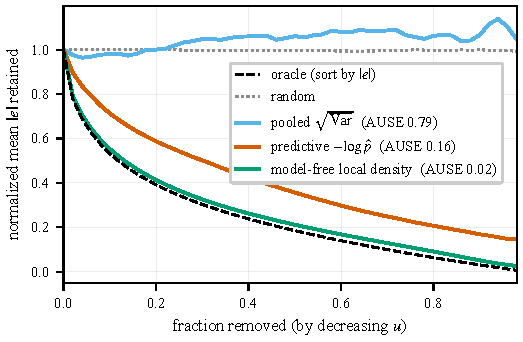
\includegraphics[width=\columnwidth]{figs/mar18_rich_sparsification.pdf}
\caption{Sparsification, March~2018, production configuration
(pipeline product): $200{,}000$ stitched-model samples scored against
the full epoch cloud (Sec.~\ref{sec:setup:metrics}); each curve
removes by its own score (the oracle by $|e|$, random uniformly).
Removing samples by decreasing predictive NLPD
tracks the error oracle far better than random removal (AUSE 0.161,
AURG 0.577); other epochs alike (Table~\ref{tab:coverage}). The
$\sqrt{\overline{\mathrm{Var}}}$ curve is the
location-queryable alternative, nearly uninformative as a ranker
(AUSE 0.786, AURG $-0.05$); the model-free local-density control
(AUSE 0.023, AURG 0.719)
outranks the NLPD ranker and nearly attains the oracle
(Sec.~\ref{sec:results:sparsification}).}
\label{fig:sparsification}
\end{figure}

On the real epochs the ranker is genuinely better than random on
every one (Table~\ref{tab:coverage},
Fig.~\ref{fig:sparsification}; production AUSE 0.161--0.205, AURG
0.521--0.577). The ranking is capacity-\emph{insensitive} (March~2018
AUSE 0.161 at $\hat{K}=841$ versus 0.165 at $\hat{K}=42$), so the
residual oracle gap is not a resolution artifact.

\looseness=-1 The signal decomposes honestly. Predictive uncertainty correlates
strongly with local point density ($\rho(u,\mathrm{density})$ of
$-0.74$, $-0.70$, $-0.67$ at production): sparser regions are genuinely
reconstructed worse, which is causally meaningful but not to be mistaken
for pure model structure.
Density-tercile stratification localizes the residual: within-tercile
AUSE is 0.28--0.50 at production, and the within-tercile gain over
random concentrates in the \emph{sparsest} tercile (AURG 0.19--0.29);
the denser terciles sit essentially at random (AURG $-0.01$ to
$0.03$), so the global ranking's power rides substantially on the
density component. The sparsest-tercile concentration holds at the reference arm as
well, so we attribute the confound to the intrinsic mismatch between
LiDAR point-density heteroscedasticity and the Gaussian likelihood
(Sec.~\ref{sec:disc-density}). For completeness, the alternative
per-point uncertainty $\sqrt{\overline{\mathrm{Var}}}$
of Sec.~\ref{sec:setup:metrics}
is nearly uninformative (AURG $-0.05$ to $+0.14$ across the six runs),
close to piecewise-constant within components. The distinction matters:
$\sqrt{\overline{\mathrm{Var}}}$ is the location-queryable uncertainty; the
predictive NLPD is an a posteriori quality-assurance instrument for
the reconstruction (Sec.~\ref{sec:setup:metrics}), not a
before-measurement error map.

\looseness=-1 The model-free control settles how much of that power is the model's
own: ranking by raw local density of the reference cloud alone
attains AUSE $0.023$--$0.024$ and AURG $0.71$--$0.72$ on the three
epochs, decisively better than the NLPD ranker, and wins within every
density tercile (AUSE $0.07$--$0.16$ vs.\ $0.28$--$0.50$); the two
orderings agree at Spearman $\rho = 0.67$--$0.74$. The NLPD ranking
is thus largely internalized sampling density, its non-density
residual adding no within-tercile power. One caveat runs in the
control's favor: $e$ is the plane distance to the same six neighbors
whose spacing defines the density, so sparse neighborhoods
mechanically inflate $e$ ($\rho$ up to $0.92$), flattering the
control's near-oracle AUSE, though the within-tercile comparison,
which coarsely controls this, still favors density. What the
predictive retains is not ranking power but form: calibrated
intervals and a ${\sim}10^{3}$-component normalized density queryable
without the $10^{7}$-point cloud (Sec.~\ref{sec:disc-density}).

\subsection{Absolute Geometric Accuracy Against the Reference Mesh}
\label{sec:results:geoacc}

\looseness=-1 The sparsification ranker is scored against the same-epoch cloud;
Table~\ref{tab:geoacc} answers the remaining absolute question:
meters against the H3D March~2018 reference mesh, in both directions,
under the protocol of Sec.~\ref{sec:setup:metrics}. Globally the
stitched model reconstructs the surface to mean $0.518$~m (median
$0.267$, RMS $0.863$, P90 $1.32$); completeness reaches $0.665$
within $0.5$~m and $0.951$ within $1$~m (the $0.25$~m fraction,
$0.254$, sits at the $0.326$~m sampling floor and is not
interpretable below it). The choice of seam rule is immaterial at this
scale: crop and Voronoi agree with the stitched model to within
$3$~mm in mean and $1.1$~mm in median in both directions (crop's
accuracy RMS runs $2.6$~cm higher, a tail effect only), consistent
with the parity of Table~\ref{tab:seam}.

\begin{table}[!t]
\caption{Geometric accuracy and completeness (meters) of the
March~2018 production fit against the H3D reference mesh, overall and
stratified by the stitched model's own predictive-NLPD terciles.
Accuracy: $197{,}508$ model samples, exact point-to-mesh distance.
Completeness: $140{,}574$ domain-masked mesh-surface samples to the
nearest of $5\times10^{5}$ model samples (resolution floor
$0.326$~m; the $\le0.25$~m fractions are floor-limited).
Completeness within $1$~m is $0.951$ overall
($1.00$/$1.00$/$0.86$ by tercile). Source:
\texttt{geoacc\_mar18.json}.}
\label{tab:geoacc}
\centering
\setlength{\tabcolsep}{4.5pt}
\begin{tabular}{lrrrrrr}
\hline
 & Mean & Med. & RMS & P90 & $\le$0.25\,m & $\le$0.5\,m \\
\hline
\multicolumn{7}{l}{\emph{Accuracy} (model $\to$ mesh)} \\
All samples & 0.518 & 0.267 & 0.863 & 1.320 & 0.479 & 0.690 \\
\enskip low NLPD  & 0.144 & 0.108 & 0.215 & 0.289 & 0.856 & 0.978 \\
\enskip mid NLPD  & 0.415 & 0.289 & 0.604 & 0.898 & 0.432 & 0.752 \\
\enskip high NLPD & 0.994 & 0.724 & 1.350 & 2.147 & 0.148 & 0.340 \\
\hline
\multicolumn{7}{l}{\emph{Completeness} (mesh $\to$ model)} \\
All samples & 0.452 & 0.380 & 0.547 & 0.821 & 0.254 & 0.665 \\
\enskip low NLPD  & 0.250 & 0.239 & 0.272 & 0.392 & 0.540 & 0.980 \\
\enskip mid NLPD  & 0.402 & 0.387 & 0.435 & 0.624 & 0.182 & 0.739 \\
\enskip high NLPD & 0.704 & 0.655 & 0.796 & 1.092 & 0.041 & 0.276 \\
\hline
\end{tabular}
\end{table}

\begin{figure}[!t]
\centering
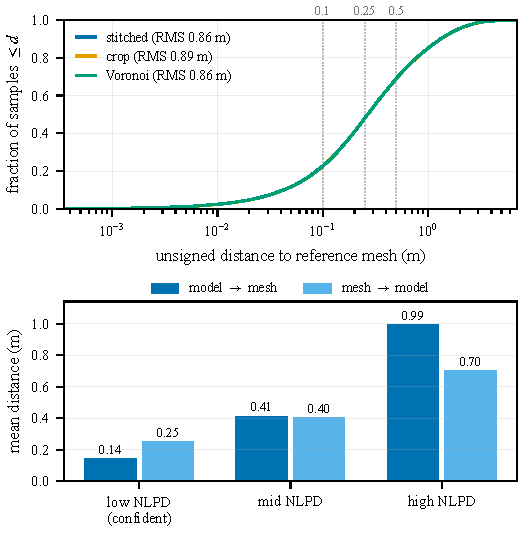
\includegraphics[width=\columnwidth]{figs/geoacc_mar18.pdf}
\caption{Geometric accuracy against the H3D March~2018 reference mesh
(pipeline product). Top: empirical CDF of unsigned model$\to$mesh
distance for the three seam rules (log axis; dotted lines at the
$0.1$/$0.25$/$0.5$~m thresholds): the rules are indistinguishable
(curves overplot to line width).
Bottom: mean distance by the stitched model's own predictive-NLPD
tercile, both directions; the stratification is monotone, and the
confident tercile is decimeter-grade.}
\label{fig:geoacc}
\end{figure}

\looseness=-1 The stratification is the operative finding
(Table~\ref{tab:geoacc}, Fig.~\ref{fig:geoacc}): ordering by the
model's own predictive NLPD (no reference data in the loop)
stratifies the error monotonically in both directions, with accuracy
tercile means of $0.144$/$0.415$/$0.994$~m. The confident third is
decimeter-grade ($85.6\%$ of its samples within $0.25$~m of the mesh,
$97.8\%$ within $0.5$~m), and the model itself identifies it.

\looseness=-1 The honest scope: these are decimeter-to-meter numbers. Classical
photogrammetric--LiDAR survey processing delivers centimeter-grade
products on data of this quality (the reference mesh itself comes
from such a chain), and the meter-band high-NLPD tail is consistent
with the ${\approx}1$~m level-of-detection floor of
Sec.~\ref{sec:results:change} (Sec.~\ref{sec:disc-lod}). What the
stitched density offers is not centimeter accuracy but a calibrated
map that knows where it is good: a self-identified decimeter-grade
core, and meter-band tails the model itself flags.

\subsection{Change Detection with a Model-Derived Level of Detection}
\label{sec:results:change}

% Synthetic slab confirmation: change_synth_slab.json (slab_summary).
The LoD$_{95}$ test of Sec.~\ref{sec:setup:metrics} applied to the
November~2018/March~2019 production fits (Fig.~\ref{fig:change}) takes
21.3~s on the
$313\times783$-cell grid ($113{,}020$ valid cells); on a synthetic 30~cm
displacement slab it attains recall 1.000, null flag rate 0.000, and
$0.06\%$ displacement error, confirming the machinery before any
real-data claim.

\begin{figure}[!t]
\centering
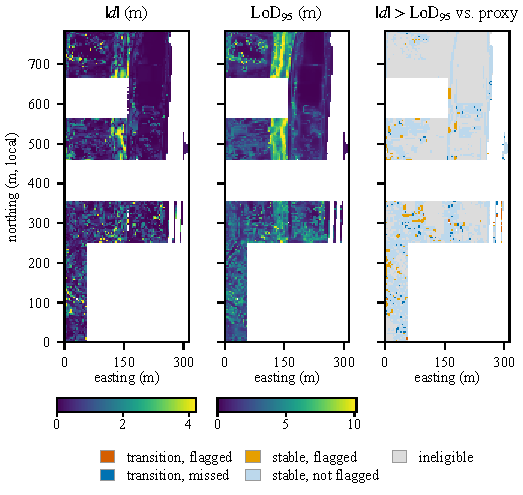
\includegraphics[width=\columnwidth]{figs/change_nov18_mar19.pdf}
\caption{Model-derived change detection, November~2018 vs.\ March~2019
(pipeline product): absolute inter-epoch elevation difference $|d|$,
per-cell LoD$_{95}$, and flagged cells against the class-transition
proxy on the 1~m grid; stable impervious cells calibrate the test
(4.2\% exceedance vs.\ nominal 5\%). White cells (all panels) have
fewer than 20 points in either epoch. Color scales are clipped at the
99th percentile; isolated flagged/transition cells are dilated by one
cell for visibility.}
\label{fig:change}
\end{figure}

\looseness=-1 \emph{Null calibration is delivered.} On the $17{,}592$ physically stable
impervious cells the exceedance rate is 4.2\% against the nominal 5\%
(median $|d|$ 0.17~m; median LoD$_{95}$ 1.16~m), insensitive to the
2~cm registration term (exceedance rate and AUC both shift by
${\sim}10^{-4}$). \emph{Detection is above chance}: on the
vegetation-excluded transition proxy (734 positives, $42{,}487$
negatives), AUC is 0.718 with recall 0.208 and precision 0.081 at the
LoD$_{95}$ threshold on 1~m cells; coarsening to 2~m cells raises AUC to
0.78 and recall to 0.35 with the null still calibrated (4.8\%), while
0.5~m cells give AUC 0.68. Across valid cells median $|d|$ is 0.28~m
(95th pct.\ 2.48~m) vs.\ median LoD$_{95}$ 1.84~m; per the
proxy caveat of Sec.~\ref{sec:setup:protocols}, the false-alarm role
belongs to the null test, not to precision at the threshold.

\begin{table}[!t]
\caption{Change detection on 1~m cells: capacity dose--response of the
model-derived test (both arms at $\sigma_{\mathrm{reg}}=0$;
high-capacity arm: $\alpha=1000$, $T=1024$, $\hat{K}=3443/3525$ for
Mar.~2019/Nov.~2018) beside the classical propagated-error DoD
on identical cells, masks, and proxy (Sec.~\ref{sec:setup:metrics}).
Sources: \texttt{change\{,\_xrich,\_classical\}\_nov18\_mar19.json}.}
\label{tab:change_dose}
\centering
\setlength{\tabcolsep}{3pt}
\begin{tabular}{lcccc}
\hline
 & \multicolumn{2}{c}{Model-derived} &
\multicolumn{2}{c}{Classical DoD} \\
 & Prod. & High cap. & $\sigma_{\mathrm{reg}}{=}0$ &
$\sigma_{\mathrm{reg}}{=}2$\,cm \\
\hline
Null exceedance (nom.\ 5\%) & 4.2\% & 0.9\% & 89.5\% & 17.1\% \\
AUC (veg-excluded)          & 0.718 & 0.776 & 0.816 & 0.973 \\
Precision at LoD$_{95}$     & 0.081 & 0.207 & 0.021 & 0.050 \\
Recall at LoD$_{95}$        & 0.208 & 0.177 & 0.984 & 0.971 \\
Median null-cell LoD$_{95}$ & 1.16~m & 1.04~m & 1.3~mm & 3.9~cm \\
\hline
\end{tabular}
\end{table}

\looseness=-1 The dose--response (Table~\ref{tab:change_dose}) settles whether more
model is the answer. Tripling capacity sharpens the test: precision
at the threshold rises from $0.081$ to $0.207$ and AUC from $0.718$
to $0.776$, at slightly lower recall ($0.177$ vs.\ $0.208$) and a
markedly more conservative null ($0.9\%$ against nominal
5\%). But the LoD floor stays at ${\approx}1.0$~m: a representation
limit (Sec.~\ref{sec:disc-lod}).

\looseness=-1 Table~\ref{tab:change_dose} also delivers the promised classical
yardstick, on literally identical cells. The propagated-error DoD
posts a far sharper nominal threshold (median null-cell LoD$_{95}$
of $1.3$~mm at $\sigma_{\mathrm{reg}}=0$, $3.9$~cm at $2$~cm, against
$1.16$~m) and, as a pure ranking score, separates the transition
proxy better (AUC $0.816$; $0.973$ with the registration term). As a
\emph{detector} it is severely anti-conservative here: $89.5\%$
($17.1\%$ with the registration term) of the stable impervious cells
exceed its nominal-5\% threshold, against $4.2\%$ for the model arm,
because the per-cell standard error shrinks as $1/\sqrt{n}$ (cells
hold hundreds of points) while inter-epoch registration and roughness
error do not. The model-derived LoD is thus deliberately
conservative (recall $0.21$ against $0.97$, with a held null) and
offers what the DoD cannot: the uncertainty rides in the fitted
mixtures, so calibrated change maps need no per-cell access to both
epochs' raw clouds at comparison time.

\subsection{Variance-Guided Re-Flight Planning}
\label{sec:results:reflight}

On the Mill~19 Rubble anchor (Sec.~\ref{sec:setup:protocols};
$1.75\times10^{6}$ points, 1{,}678 images) the re-flight experiment
asks whether the model's own posterior can plan the next flight; all
arms are scored on one frozen evaluation set that no refit ever sees
(Table~\ref{tab:reflight}). The null control frames the block
scenarios: with held-back imagery \emph{interleaved} through the
survey, no planner, including the error oracle, moved held-out NLPD
by more than $0.04$~nats at a 20\% or 50\% dose: re-flying covered
ground buys nothing; the operational case is contiguous \emph{new}
ground.

\begin{table}[!t]
\caption{Re-flight planning on Mill~19 Rubble (block holdback, new
ground): improvement in mean held-out NLPD (nats; baseline $-$ arm),
overall and within the granted tiles. Random arms: mean $\pm$ sample
s.d.\ over seeded replicates. $^{\dagger}$Selects the same tiles
as expected yield, so the rows coincide.
$^{\ddagger}$Selects the same tiles as the error oracle (row
omitted as a duplicate). Sources:
\texttt{reflight\_rubble\_*\_v2.json},
\texttt{reflight\_rubble\_mass\{6,12\}.json}.}
\label{tab:reflight}
\centering
\setlength{\tabcolsep}{4pt}
\begin{tabular}{llrr}
\hline
Scenario & Planner & $\Delta$ overall & $\Delta$ granted \\
\hline
Block, 6 tiles    & uncertainty$^{\ddagger}$ & $+1.10$ & $+1.90$ \\
(2 grants)        & mass only          & $+0.86$ & $+1.37$ \\
                  & random (5 seeds)   & $+0.45 \pm 0.17$ & $+1.45 \pm 0.54$ \\
\hline
Block, 12 tiles   & raw NLPD ranking   & $+0.14$ & $+1.88$ \\
(3 grants)        & expected yield     & $+1.15$ & $+1.45$ \\
                  & mass only$^{\dagger}$ & $+1.15$ & $+1.45$ \\
                  & error oracle       & $+0.55$ & $+1.96$ \\
                  & random (8 seeds)   & $+0.46 \pm 0.42$ & $+1.15 \pm 0.52$ \\
\hline
\end{tabular}
\end{table}

\looseness=-1 \emph{Act 1: posterior uncertainty finds where the model is wrong.} On
the 6-tile site grid, with the unfinished 20\% strip held back, the
uncertainty
planner selects exactly the tiles the error oracle selects and
improves held-out NLPD by $+1.10$~nats, above every random grant
($+0.45\pm0.17$, 5 seeds; best $+0.61$); the gain is local, not drift
($+1.90$ inside the granted tiles). It also beats the mass-only
control, which grants 8\% more points ($128{,}344$ vs.\ $118{,}730$)
yet achieves only $+0.86$: the posterior finds \emph{which}
comparable-mass ground is badly modeled, not merely \emph{where} data
are recoverable.

\looseness=-1 \emph{Act 2: raw uncertainty is mass-blind.} On the finer 12-tile grid,
ranking tiles by raw mean NLPD still targets genuinely bad tiles
($+1.88$ inside its grants) but selects tiles with almost no
recoverable imagery: it grants only $19{,}734$ pool points and moves
the overall score by $+0.14$, below the random mean of
$+0.46\pm0.42$ (seed range $+0.00$ to $+0.99$).

\looseness=-1 \emph{Act 3: where mass separates tiles, mass dominates.} Scoring tiles by \emph{expected yield} (mean tile NLPD $\times$
grantable pool mass; the NLPD factor is available before flying, while
the mass factor, measured here from the held-back block, stands in for
the coverage-based yield estimate a planner would form in advance)
resolves the failure:
$+1.15$~nats held-out (Table~\ref{tab:reflight}), above all eight
random draws (best $+0.99$), and raises the fraction of evaluation
points within $0.5$~m of a model sample by $+0.09$. But so does recoverable mass alone: the mass-only control
selects the identical tiles and matches $+1.15$ exactly. On this grid
the posterior factor adds no selection signal, and the margin over
the error oracle (itself at $+0.55$) is carried by the mass term: the oracle's
grants carry $62{,}387$ pool points against the yield planner's
$157{,}739$. Read together with Act~1: mass is the first-order
planning signal, and the posterior's measured value concentrates
exactly where mass stops discriminating.

% Section VI: Discussion / Limitations
% All numbers trace to PHASE_B_FINDINGS.md / experiments/out/*.json (see OUTLINE.md §VI).

\section{Discussion and Limitations}
\label{sec:discussion}

\subsection{What the Stitched Density Does and Does Not Buy}
\label{sec:disc-stitch}

\looseness=-1 Table~\ref{tab:seam} is deliberately a parity result. Stitching does
\emph{not} buy nats: a practitioner needing only a rasterized product
loses nothing by cropping. It buys the object itself, a normalized
global density with every fitted component's evidence intact and
duplication resolved by an explicit exact merge, not implicit
deletion. The crop baseline is moreover charitable (globally
renormalized, where deployed pipelines skip it), and deletion's
near-zero cost is an empirical fact of these scenes, not a guarantee:
it grows in principle with the mass straddling seams, a regime this
study does not test. The second site cuts the other way too: SMBU's production
seam bands show a $-0.37$-nat stitched deficit and 68\% seam coverage
of $0.570$ (Secs.~\ref{sec:results:seams}--\ref{sec:results:calibration}),
so neither seam parity nor seam calibration of the stitched rule
travels automatically across sites; both must be checked per campaign.

\subsection{The Level-of-Detection Floor Is Intrinsic}
\label{sec:disc-lod}

\looseness=-1 The change-detection level of detection saturates at approximately
$1.0$~m and no configuration we tried lowers it: the floor survives
the ${\sim}3\times$ capacity increase of Table~\ref{tab:change_dose},
cell sizes 0.5--2~m, and a 2~cm registration term, even as ranking
and precision improve. We conclude it is a representation limit of
Gaussian mixtures on heterogeneous urban vertical structure: roof
edges, facades, and vegetation within one component's support inflate
the posterior mean-location variance the LoD is built from. We
expect no tuning to remove it; sub-meter sensitivity would require a
likelihood modeling vertical layering explicitly. The floor is
consistent with the measured absolute accuracy: model-to-mesh error is
decimeter-grade only in the confident tercile and meter-band in the
worst (Sec.~\ref{sec:results:geoacc}), an order of magnitude above the
centimeter grade classical survey processing achieves on data of this
quality. For the LoD itself the classical yardstick is now measured
(Sec.~\ref{sec:results:change}): the same-grid propagated-error DoD
posts nominal mm--cm thresholds but flags 17--90\% of stable ground,
so the ${\approx}1$~m floor is the price of a held null level here,
not mere bluntness; whether a full M3C2-EP error budget with
explicitly modeled alignment
uncertainty~\cite{winiwarter2021m3c2ep} can hold the null at
centimeter LoDs is the open classical arm (Sec.~\ref{sec:disc-open}).

\subsection{The Density Component of the Uncertainty Signal}
\label{sec:disc-density}

\looseness=-1 As quantified in Sec.~\ref{sec:results:sparsification}, the
predictive-NLPD error ranking is largely internalized sampling
density (a model-free density ranker outranks it, with rank
agreement $\rho = 0.67$--$0.74$), and the within-tercile gain over
random concentrates in the sparsest tercile; the pattern's
replication across a $20\times$ capacity change makes this intrinsic
to the mismatch between LiDAR sampling heteroscedasticity and the
Gaussian observation model, not a resolution artifact. An operator
holding the raw cloud should rank by density; what the predictive
adds is the calibrated, compact form
(Sec.~\ref{sec:results:sparsification}), and its ranking should be
read as ``sparse and poorly explained,'' not as a density-free
model-error signal.

\subsection{What $\hat{K}$ Is and Is Not}
\label{sec:disc-khat}

\looseness=-1 We report the deconfounding of $\hat{K}$ as a finding. On the STPLS3D
matched-$N$ grid (29 scenes $\times$ $\alpha\in\{0.1,1,10\}$ $\times$
2 seeds, all at $N=3\times10^{6}$ points), realized complexity at
$\alpha=1$ falls in the narrow band $\hat{K}\in[18,25]$ from empty
terrain to dense urban, with no content signal:
$\rho(\hat{K},\text{class-entropy})=0.13$ ($p=0.34$),
$\rho(\hat{K},\text{surface variation})=-0.04$,
$\rho(\hat{K},\text{density})=0.00$; the $\alpha=10$ arm is
truncation-pinned at $T=64$, and a prior length-scale sweep (29
scenes $\times$ three scale factors, $0.03$--$0.3\times$ the default,
at $\alpha=1$ and a single seed; the main grid's default-scale arm
supplies the $1\times$ endpoint) leaves per-scene $\hat{K}$ unchanged to
within one component (5 of 29 scenes shift by exactly $\pm1$). In
total 261 controlled fits, the $174$-fit matched-$N$ grid plus the
$87$-fit sweep: under
truncated stick-breaking CAVI at matched $N$, realized complexity is
set by component-death dynamics and data volume, consistent with the
base model's asymptotics~\cite{dong2026dpsplat}; on the H3D tiles,
$\rho(\hat{K},\text{tile point count})=0.97/0.82/0.85$ (full-epoch
reference fits; production refits $0.77$--$0.98$). We claim
$\hat{K}$ only as automatic, data-volume-adaptive capacity
control (useful, since a fixed budget as in
VBGS~\cite{vandemaele2024vbgs} over-provisions empty tiles and starves
dense ones, Fig.~\ref{fig:khat_deconfound}) and disclaim any reading
of $\hat{K}$ as a map of scene content.

\begin{figure}[t]
  \centering
  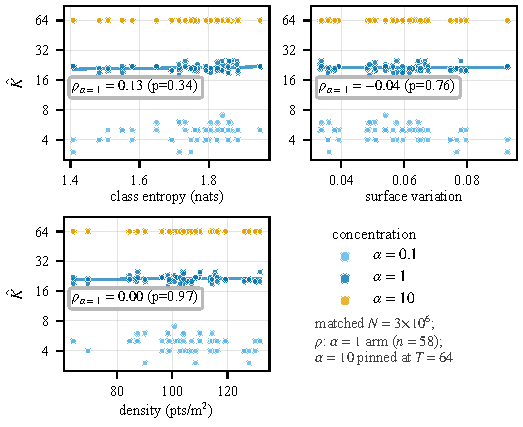
\includegraphics[width=\columnwidth]{figs/stpls3d_khat_vs_complexity.pdf}
  \caption{$\hat{K}$ against scene-content descriptors on the STPLS3D
  matched-$N$ grid (pipeline product; 29 scenes $\times$ 2 seeds per
  concentration arm, annotated $\rho$ and least-squares trend lines
  from the $\alpha{=}1$ arm;
  surface variation is the local-PCA smallest-eigenvalue ratio
  $\lambda_{\min}/\sum_i \lambda_i$ over $k{=}16$ nearest neighbors in
  a fixed $5{\times}10^{4}$-point uniform subsample per scene): the
  association is null, while the $\alpha{=}10$ arm is
  truncation-pinned at $T{=}64$; on real tiled scenes $\hat{K}$
  tracks per-tile point count ($\rho$ up to $0.98$,
  Sec.~\ref{sec:disc-khat}).}
  \label{fig:khat_deconfound}
\end{figure}

\subsection{Scope of the Re-Flight Study}
\label{sec:disc-anchor}

\looseness=-1 The Mill~19 planning results rest on a sparse COLMAP
anchor~\cite{turki2022meganerf}: a planning-scale demonstration on
held-back imagery, with no flights executed and no absolute-scale claims
beyond the anchor's metric coherence. The mass-only control (grant by
pool mass, ignoring the model) has been run in both scenarios
(Sec.~\ref{sec:results:reflight}): the posterior factor is dispensable
for mass-separable grants and demonstrably valuable for
mass-comparable ones; whether that margin persists on dense
photogrammetric products is left to future work
(Sec.~\ref{sec:conclusion}).

\subsection{Open Protocol Questions}
\label{sec:disc-open}

\looseness=-1 Cross-tile merge acceptance is rare at $10^{7}$-point tiles under
$\alpha=1$ (Sec.~\ref{sec:results:seams}), consistent with dominance
of the likelihood term in the sign test at large $N$
(Sec.~\ref{sec:merge}); a halo-width and acceptance-threshold ablation
with an ELBO-based criterion is left to future work, as are
hierarchical Dirichlet-process (HDP) sharing across tiles, a spatially
blocked hold-out
protocol (Sec.~\ref{sec:setup:protocols}), a full M3C2-EP error
budget on the same cells (the plain propagated-error DoD arm is
measured in Sec.~\ref{sec:results:change}), and
external validation of the class-transition change proxy. Finally, we
claim no theoretical seam-coverage guarantee: calibration is an
empirical, per-campaign check
(Secs.~\ref{sec:results:calibration}, \ref{sec:disc-stitch}).

% Section VII: Conclusion
% Numbers trace to PHASE_B_FINDINGS.md / experiments/out/*.json (see OUTLINE.md §VII).

\section{Conclusion}
\label{sec:conclusion}

\looseness=-1 Partition-of-unity stitching with exact conjugate merging turns
independent per-tile posteriors into a single normalized,
provenance-preserving predictive density that matches crop/Voronoi
seam deletion on held-out quality (within $0.02$--$0.03$~nats/point on
three H3D epochs) while deleting nothing, with near-nominal coverage
including at seams; at the second site, overall parity and all-points
calibration replicate while the seam bands fall short, and we say so.
That normalized density, not a nat advantage, is
the contribution: it makes the calibrated intervals, NLPD error
ranking, model-derived level of detection, and acquisition score
well-defined, and it pays where spent: predictive confidence
stratifies mesh-referenced accuracy monotonically, isolating a
self-identified decimeter-grade core ($0.14$~m mean vs.\ $0.52$~m
overall); the model-derived LoD holds its null where a same-grid
classical DoD flags 17--90\% of stable ground (though the DoD remains
the sharper pure ranker); posterior-guided
re-flight
matches a per-tile error oracle and beats a mass-only control on
comparable-mass grants ($+1.10$ vs.\ $+0.86$~nats), with the
mass-dominated regime attributed, and the exact merge is what holds
the stitched density at seam parity ($+0.14$--$0.35$~nats at seams in
ablation). All of this runs on a laptop at $10^{8}$-point
scale. Future work: halo-width and merge-threshold
ablations, a full M3C2-EP error budget for the change test, HDP
cross-tile sharing, and a GPU dense phase extending to
photogrammetric sources with LiDAR-referenced validation on
GauU-Scene.


\section*{Data and Code Availability}
\looseness=-1 All four datasets are publicly accessible from their
originators~\cite{koelle2021h3d,turki2022meganerf,chen2022stpls3d,xiong2024gauuscene}
under the access and license terms noted per dataset in
Sec.~\ref{sec:setup:datasets}. In keeping with
the non-commercial license terms, no derived point clouds or
fitted models are redistributed; the complete pipeline, configuration,
evaluation scripts, and aggregate result records reproducing every
number and figure from the original data are available at
\url{https://github.com/archiedong/dp-splat-uav}.

\bibliographystyle{IEEEtran}
% Final-page balance: at the current reflow the reference list exactly
% fills page 13 and the page is full, so no \IEEEtriggeratref is
% needed. Re-add one (standard IEEEtran device) if the reference list
% or preceding text changes.
% Page-count ruling (round 1): body plus references occupy pages 1-13;
% the IEEEbiographynophoto block alone overflows to page 14, accepted
% for the submission draft (bio pages are commonly set aside from the
% technical-page budget).
% Page-count ruling (round 5): re-examined. All 26 columns of pp. 1-13
% are flush-full; every paragraph on pp. 12-13 with a recoverable short
% last line already carries \looseness=-1; IEEEtran's bibliography
% itemsep is already zero. Lines saved upstream (verified with
% \looseness=-1 probes in Secs. III/IV, since reverted) are absorbed by
% float-separation stretch at the p11/p12 boundary and never reach
% p13, so the ~5-line deficit for the bio cannot be recovered without
% cutting content or violating class defaults. Left at 14 pages.
\bibliography{references}

\begin{IEEEbiographynophoto}{Aqi Dong}
is with the Department of Management, Marketing and Operations, David B.
O'Maley College of Business, Embry-Riddle Aeronautical University, Daytona
Beach, FL, USA. His research interests include Bayesian nonparametric
methods, variational inference, and uncertainty quantification for
three-dimensional scene representations and geospatial analytics.
% PI-OPTIONAL: a degrees line ("He received the ... degree from ... in ...")
% can be added here if desired.
\end{IEEEbiographynophoto}

\end{document}
